\chapter{Clustering}
\section{Introduction to Clustering}
Supervised learning which is the most common type of learning problem [\cite{ref71}] is also very popular in text mining [\cite{ref245}]. In order to successfully solve the problems belonging to the supervised learning category, the texts to be processed need to have assigned labels that describe the categories in the data. A supervised learning algorithm can, using the documents' properties and labels, generalize what documents in categories look like, what is typical for them, and how to correctly assign unlabeled instances to one or more existing categories.

Unfortunately, unavailability of the labelled data is often a major problem in text mining [\cite{ref228}]. It is because the labeling process itself is very demanding. Reading tens or hundreds of documents and correctly assigning labels to them requires the effort of many people for many hours. Even when the human annotators are experts in the given field, the resulting quality of the labeling process is not have to always be high. It is not uncommon that a complete agreement of the annotators is not achieved [\cite{ref239}]. Additionally, new data constantly occurs, so it is nearly impossible to have the labels assigned to the data in a reasonable time and in reasonable amounts.

\textit{Clustering} is the most common form of unsupervised learning and enables automatic grouping of unlabeled documents into subsets called clusters. It is expected that the clusters are homogeneous internally and can be clearly distinguished from the others. This means that the documents contained in one cluster are more similar (e.g., share the same topic) to the remaining documents in the same cluster than to the documents in the other clusters. Here, we might anticipate that the document properties together with the concept of similarity play a crucial role in the clustering process.

Clustering has gained in importance with the increasing amounts of data available. It covers a wide variety of algorithms rooted in statistics, computer science, computational intelligence, and machine learning with applications in many disciplines [\cite{ref285}].

Clustering has frequently been used successfully for organizing and searching large text collections, for example, in automatic creation of ontologies, summarizing, disambiguating, and navigating the results retrieved by a search engine, patent analysis, detecting crime patterns and many others [\cite{ref61}, \cite{ref70}, \cite{ref262}, \cite{ref108}, 
\cite{ref40}]. If the clusters are good and reliable with respect to the given goal, they can be successfully used as classes or in order to improve classification [\cite{ref84}, \cite{ref158}].

\section{Difficulties of Clustering}
In supervised learning tasks, the goal is usually well defined and described. For example, in a spam filtering problem, we want to separate spam e-mails from the relevant ones. What spam e-mails look like can be derived from a collection of good examples of spam. Then, a learning algorithm looks at the properties of spam e-mails and compares them with the properties of other e-mails. The relevant properties that can be used in distinguishing spam from the rest are somehow combined in the model (e.g., in the tests contained in the nodes of a decision tree) or in the measures quantifying their relationship to a category are determined (e.g., the probabilities in the naïve Bayes classifier). The success of the generalization can be measured by clearly defined measures like the correctness of classification. Unfortunately, one clear answer to a clustering problem and measures that indisputably evaluate the outcomes of unsupervised learning tasks do not exist.

Imagine an example from the clothing industry. We have information about the physical characteristics of our customers and we want to determine the suitable sizes of the clothes, take T-shirts, for instance. Since we have no information about the sizes to be made, we want to find groups of people with similar physical characteristics and to offer one size for each group. As the people in one group are expected to be similar, we hope the size will fit all of them. The question is, how many groups should we define? A larger number of available sizes will be appreciated by the customers but will put additional requirements on our business (developing more sizes, manufacturing more different sizes, keeping more sizes in stock, etc.). Having a lower number of models will make the business easier but can discourage the customers who do not find the perfect size. One extreme is to make only one size and provide it to all, the other possibility is to manufacture a unique size for each customer. All mentioned options are good from some perspective. At the same time, all of them are not good for some other reasons. It is therefore obvious that no single correct answer exists and that it depends on the problem that is to be solved and how the problem is evaluated. When empha-sizing the convenience of the customers, more sizes should be provided. When the ease of the business has a higher importance, a lower number of T-shirt sizes would be preferred.

We might relate similar considerations to text documents; for example, newspaper articles. Clustering can be used in order to find groups of similar articles, sharing a common topic. This may be useful in an information retrieval task when relevant documents matching a user defined query should be returned. Clustering can be applied to the documents before retrieval, so groups of similar documents are found. These groups are represented by their centroids and every search request is first compared to the centroids. Subsequently, matching the query against documents is carried out only in the selected, highly relevant groups [\cite{ref234}]. A question similar to the one on the T-shirts example arises here: How many groups of documents should be created?

Having more clusters means that they are more specific. For example, instead of one group containing documents related to sports, we may have more groups focused on football, ice hockey, athletics, the Winter Olympic Games, The National Hockey League, etc. More clusters will probably result in a more efficient way of retrieving the documents because a smaller number of documents needs to be compared to the query. The precision, i.e., the percentage of relevant documents, will most likely be higher because the clusters should contain documents that are somewhat similar and thus sharing a common topic. On the other hand, the recall, measuring the portion of relevant documents that have been retrieved, could be lower because some other clusters might also contain relevant documents, but other topics are prevailing there.

When the created clusters are to be used for subsequent classification we have to realize that it will be easier to distinguish documents about sports from other categories, the economy, politics, or nature, for instance. It will be more complicated to differentiate between documents about tennis, badminton, and table tennis, representing quite similar topics under the sports category.

Sometimes, information about the relationships between clusters, for example, knowing that groups of documents talking about athletics and football belong to another group talking about sports, might be interesting too. This means that a clustering technique that is able to produce a hierarchy of clusters is suitable in this situation.

It is obvious that there might be many goals and evaluation viewpoints. Thus, interesting structures in the document collection are expected to be found [\cite{ref274}] and the evaluation must be often done by a human expert. There are also many measures which can be considered in the evaluation process that somehow quantify the properties of the created clusters (i.e., measure the quality of clustering).

\section{Similarity Measures}
Document similarity is the only endogenous information that is available in the clustering process. The similarity can be measured between individual documents, between groups of documents, or between a document and a group of documents. It is therefore necessary to define how to represent a group of documents. One of the possibilities is to represent a group of documents using its centroid (i.e., the average document):


\begin{equation*}
\text { Centroid }_{C}=\frac{\sum_{x \in C} x}{|C|}, \tag{12.1}
\end{equation*}


where $|C|$ is the number of documents in cluster $C$. A cluster can also be represented by one of the documents contained in it, for example, by its medoid (a document closest to the centroid). All this depends on the applied clustering algorithm. For instance, some algorithms measure the similarity between two clusters in terms of the similarity of the most similar objects (single linkage clustering method) or two most dissimilar objects (complete linkage clustering method). In the k -means algorithm, the objects are moved to the closest cluster which is determined according to the proximity to a cluster centroid. In agglomerative centroid methods, each cluster is represented by a centroid and the similarity is calculated between these centroids [\cite{ref230}, \cite{ref128}].

Let a measure $d\left(x_{1}, x_{2}\right)$ represent the distance between objects $x_{1}$ and $x_{2}$. If it should be considered a correct metric, the following criteria must be fulfilled [\cite{ref242}, \cite{ref283}, \cite{ref250}]:

\begin{itemize}
  \item $d\left(x_{1}, x_{2}\right) \geq 0$, i.e., the distance is always non-negative;
  \item $d\left(x_{1}, x_{2}\right)=0$ if $x_{1}$ and $x_{2}$ are identical which is known as self-proximity;
  \item $d\left(x_{1}, x_{2}\right)=d\left(x_{2}, x_{1}\right)$ which means that the distance must be symmetrical;
  \item $d\left(x_{1}, x_{2}\right) \leq d\left(x_{1}, x_{3}\right)+d\left(x_{3}, x_{2}\right)$ which is known as the triangle inequality.
\end{itemize}

If we look, for example, at the cosine similarity measure we can see that some of the conditions are violated. Thus, similarities are sometimes converted to distances using some simple monotonic function such as the linear transform or the inverse transform [\cite{ref130}]:


\begin{align*}
\operatorname{Sim}_{\text {linear }}\left(x_{1}, x_{2}\right) & =C-\operatorname{Dist}\left(x_{1}, x_{2}\right)  \tag{12.2}\\
\operatorname{Sim}_{\text {inverse }}\left(x_{1}, x_{2}\right) & =\frac{1}{\operatorname{Dist}\left(x_{1}, x_{2}\right)+C} \tag{12.3}
\end{align*}


where $C$ is a constant that enables the fitting of the similarity values to a desired interval.

Although the terms similarity and distance are sometimes used interchangeably, there is a difference between them. If, for example, two points in the space are close to each other, their distance is low, but their similarity is high. If the two points are identical, their distance is minimal (zero) and their similarity is maximal (typically 1). Thus saying, for example, that the Euclidean distance is used as a similarity measure or that the cosine similarity measures the distance between two vectors is not completely correct.

There are many possibilities of measuring the similarity between documents. They typically consider the values of the attributes of the compared documents and combine the outcome of the comparison into a single value. This value reflects the positions of the documents in the multidimensional space. The position can be perceived as single points or as a vector with the beginning in the origin of the space (the point $(0,0,0, \ldots, 0)$ ) and ending in that point. Generally, the closer the points or vectors appear, the more similar the documents are. Given examples of what is similar and what is not, it is also possible to learn a new distance metric that takes these requirements into consideration [\cite{ref283}].

\subsection{Cosine Similarity}
In text mining tasks, cosine similarity based on the angle $\theta$ between vector pairs is very popular [\cite{ref138}]. It is calculated as the cosine of the angle $\theta$ between two vectors $x_{1}$ and $x_{2}$ :


\begin{equation*}
d_{\text {cosine }}\left(x_{1}, x_{2}\right)=\cos (\theta)=\frac{x_{1} \cdot x_{2}}{\left\|x_{1}\right\|\left\|x_{2}\right\|}=\frac{\sum_{i=1}^{m} x_{1}^{i} \cdot x_{2}^{i}}{\sqrt{\sum_{i=1}^{m}\left(x_{1}^{i}\right)^{2}} \cdot \sqrt{\sum_{i=1}^{m}\left(x_{2}^{i}\right)^{2}}}, \tag{12.4}
\end{equation*}


where $x_{1} \cdot x_{2}$ is the dot (linear, scalar) product of vectors $x_{1}$ and $x_{2}$ and $\left\|x_{i}\right\|$ is the length of vector $x_{i}$. The dot product has a favourable property which makes it popular for calculating similarities. If the values of $i^{t h}$ attribute of $x_{1}$ and $x_{2}$ are not zeros (i.e., the documents share the same property, e.g., a word) the value of the dot product will be bigger. If one document has a certain property ( $x_{1}^{i}>0$ ) and the other not $\left(x_{2}^{i}=0\right)$ the value of the dot product will not increase because $x_{1}^{i} \cdot x_{2}^{i}=0$.

The problem of the dot product is that longer vectors, i.e., vectors containing more values, cause the dot product to be higher. When the vectors are normalized to a unit vector (a vector with size 1) their dot product is then equal to the cosine of the angle between them. When the vectors are already normalized (we can achieve this by dividing the vectors by their lengths), the cosine similarity can be simply calculated as


\begin{equation*}
d_{\text {cosine }}\left(x_{1}, x_{2}\right)=x_{1} \cdot x_{2} \tag{12.5}
\end{equation*}


The values of the cosine similarity range from 0 to 1 as the angle between the vectors can be between 0 and 90 degrees (we consider only that part of the vectors space where the attribute values are positive because the weights in document vectors are always positive - a document cannot contain a certain word a negative number of times). The more similar the documents are, the smaller the angle between their vectors is, so the value of this measure is higher.

The cosine similarity does not satisfy the conditions of being a metric. This can be easily solved by working with the angle between two vectors, not with its cosine [\cite{ref242}]:


\begin{equation*}
d_{\text {cosine }}\left(x_{1}, x_{2}\right)=\arccos \frac{\sum_{i=1}^{m} x_{1}^{i} \cdot x_{2}^{i}}{\sqrt{\sum_{i=1}^{m}\left(x_{1}^{i}\right)^{2}} \cdot \sqrt{\sum_{i=1}^{m}\left(x_{2}^{i}\right)^{2}}} \tag{12.6}
\end{equation*}


The $\arccos$ function (a function inverse to $\cos$ ) gives us the angle from its cosine. The angle can be between 0 and $\pi / 2$ so if we want to normalize the value of the distance measure (to keep the values between 0 and 1 ), we can simply divide it by $\pi / 2$. To avoid complicated calculations of the $\arccos$ function, we can calculate the cosine distance as 1 - similarity [\cite{ref91}].

\subsection{Euclidean Distance}
The Euclidean distance is a standard geometric distance measuring the distance of two points in an $n$-dimensional space (in a two or three dimensional space, it can easily be measured by a ruler). It is the implicit distance for the k -means algorithm [\cite{ref120}].


\begin{equation*}
d_{\text {Euclidean }}\left(x_{1}, x_{2}\right)=\sqrt{\sum_{i=1}^{m}\left(x_{1}^{i}-x_{2}^{i}\right)^{2}} \tag{12.7}
\end{equation*}

\subsection{Manhattan Distance}
Manhattan distance is also known as city block distance, according to the distance you need to walk between two places using only orthogonal streets (the name comes from the island of Manhattan where the streets are mostly organized into a rectangular grid). The distance is simply calculated as the sum of differences across all dimensions [\cite{ref97}]:


\begin{equation*}
d_{\text {Manhattan }}\left(x_{1}, x_{2}\right)=\sum_{i=1}^{m}\left|x_{1}^{i}-x_{2}^{i}\right| \tag{12.8}
\end{equation*}


\begin{figure}[H]
\begin{center}
  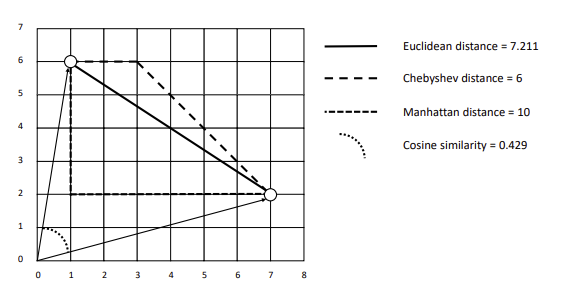
\includegraphics[width=0.8\textwidth]{chapter/chapter12/figure12_1.png}
\captionsetup{labelformat=empty}
\caption{\textbf{Figure 12.1:} A graphical representation of selected similarity measures.}
\label{fig12.1}
\end{center}
\end{figure}

\subsection{Chebyshev Distance}
Chebyshev distance is also known as maximum distance or chessboard distance, according to the number of moves a king on a chessboard must make when moving from one place to another in the shortest way. It is calculated as the maximum from differences across all dimensions [\cite{ref284}]:


\begin{equation*}
d_{\text {Chebyshev }}\left(x_{1}, x_{2}\right)=\max _{i=1}^{m}\left|x_{1}^{i}-x_{2}^{i}\right| \tag{12.9}
\end{equation*}

\subsection{Minkowski Distance}
This distance is a generalization including the Euclidean, Manhattan, and Chebyshev distances. The specific form of the distance depends on the parameter $p$ known as the order:


\begin{equation*}
d_{\text {Minkowski }}\left(x_{1}, x_{2}\right)=\sqrt[p]{\sum_{i=1}^{m}\left(x_{1}^{i}-x_{2}^{i}\right)^{p}}, p \geq 1 \tag{12.10}
\end{equation*}


If $p$ is 1 , we have the Manhattan distance, $p=2$ gives us the Euclidean distance, and $p=\infty$ represents the Chebyshev distance [\cite{ref16}].

\subsection{Jaccard Coefficient}
The Jaccard coefficient measures the similarity in terms of intersection of two sets divided by their union. For text documents, the Jaccard coefficient compares\\[0pt]
the sum of weights of shared terms to the sum of weights of terms that are present in either of the two documents but are not the shared terms [\cite{ref120}]:


\begin{align*}
d_{\text {Jaccard }}\left(d_{1}, d_{2}\right) & =\frac{d_{1} \cdot d_{2}}{\left\|d_{1}\right\|+\left\|d_{2}\right\|-d_{1} \cdot d_{2}} \\
& =\frac{\sum_{i=1}^{m} d_{1}^{i} \cdot d_{2}^{i}}{\sqrt{\sum_{i=1}^{m}\left(d_{1}^{i}\right)^{2}}+\sqrt{\sum_{i=1}^{m}\left(d_{2}^{i}\right)^{2}}-\sum_{i=1}^{m} d_{1}^{i} \cdot d_{2}^{i}} \tag{12.11}
\end{align*}

\section{Types of Clustering Algorithms}
We have a set, $X=\left\{x_{1}, x_{2}, \cdots, x_{n}\right\}$, of documents to be clustered, as the input. There are various algorithms which have a common goal - to assign the documents to appropriate clusters. The methods generally differ in the way of representing the similarities between documents and finding the clusters. The algorithms might be based on distances, probabilities, density, and other measures. The earliest methods of document clustering, like the k -means algorithm and agglomerative methods, were based on distances [\cite{ref5}].

When an algorithm assigns each object to exactly one cluster, we talk about hard clustering. It is also possible to have each object associated with each cluster with a degree of membership in the interval $[0,1]$. This approach is known as soft or fuzzy clustering [87]. Sometimes, a document does not have to be assigned to a cluster. This is called non-exhaustive clustering [\cite{ref277}].

Clustering algorithms usually operate on two types of structures. The first type represents the objects to be clustered as sequences of objects' attributes (variables, features) in the form of vectors $x_{i}=\left(x_{i}^{1}, x_{i}^{2}, \cdots, x_{i}^{m}\right)$. All objects then form an object-by-variable matrix (e.g., a term-document matrix). The second structure is a collection of proximities that have to be available for all pairs of the objects. The proximities are then represented by a square object-to-object matrix containing similarities or dissimilarities of the objects [\cite{ref142}].

\subsection{Partitional (Flat) Clustering}
The goal of partitional (flat) clustering is to find a partition $C=\left\{C_{1}, C_{2}, \cdots, C_{k}\right\}$, $k \leq n$ of $X$ such that every document belongs to one and only one set of $C$ that are called clusters. This means, that the clusters are not overlapping and their union gives us the set $X$. Partitioning clustering can be formally described as follows [\cite{ref285}]:


\begin{gather*}
C_{i} \neq \emptyset, \quad i=1,2, \cdots, k \\
\bigcup_{i=1}^{k} C_{i}=X  \tag{12.12}\\
C_{i} \cap C_{j}=\emptyset, \quad i, j=1,2, \cdots, k \text { and } i \neq j
\end{gather*}


During flat clustering, the value of an objective function that quantifies the quality of a clustering solution is optimized. The objective function usually describes how similar the documents and the cluster centroids are, how dissimilar the centroids are, and so on; see below.

It is not computationally feasible to use brute force to examine all possible clustering solutions to find the best one. Thus, flat clustering usually starts with an initial solution based on some random element (the seed) and this solution is further improved in several iterations. When the initial solution is not well selected, the final partitioning does not have to be optimal (the search process does not reach the global optimum). Thus, some methods of pre-computing the seed to increase the chance of reaching the global optimum might be employed.

\subsection{Hierarchical Clustering}
Hierarchical clustering constructs a tree-like structure (hierarchy) $H= \left\{H_{1}, H_{2}, \cdots, H_{h}\right\}$ of subsets $H_{i} \subseteq X$ such that any two sets $H_{i}$ and $H_{j}$ are either disjoint or one contains the other. The clusters at the bottom of this hierarchy contain only a single object from $X$ (singleton clusters). One of the subsets, the root of the hierarchy, contains all clustered objects. Mathematically hierarchical clustering is described as [\cite{ref197}]:


\begin{gather*}
H_{i} \subset H_{j}, H_{j} \subset H_{i} \text { or } H_{i} \cap H_{j}=\emptyset \text { for any } i, j=1,2, \cdots, h, \text { and } j \neq i \\
\{x\} \in H \text { for each } x \in X  \tag{12.13}\\
X \in H
\end{gather*}


Two approaches can be applied when building the hierarchy of clusters -top-down in case of divisive hierarchical clustering and bottom-up in agglomerative hierarchical clustering. While agglomerative algorithms are strictly local, meaning that they consider only the closest neighbourhood of clusters, divisive algorithms are more global because the context of all data has been, in some way, used so far when partitioning a cluster into subsets [\cite{ref3}].

The result of hierarchical clustering can be visualized using a dendrogram where the proximity of individual objects as well as the clusters is well visible. A dendrogram over a set $X$ is a binary rooted tree where the leaves correspond to

\begin{figure}[H]
\begin{center}
  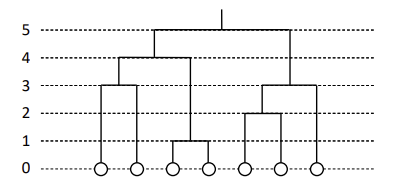
\includegraphics[width=0.8\textwidth]{chapter/chapter12/figure12_2.png}
\captionsetup{labelformat=empty}
\caption{\textbf{Figure 12.2:} A dendrogram with levels [3].}
\label{fig12.2}
\end{center}
\end{figure}

\begin{figure}[H]
\begin{center}
  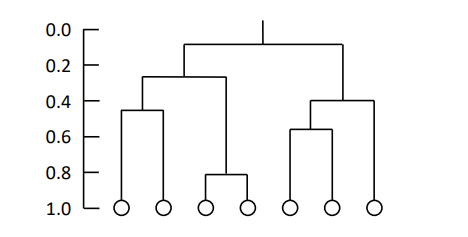
\includegraphics[width=0.8\textwidth]{chapter/chapter12/figure12_3.png}
\captionsetup{labelformat=empty}
\caption{\textbf{Figure 12.3:} A dendrogram with combination similarities [185].}
\label{fig12.3}
\end{center}
\end{figure}

the elements of X . Every node is assigned a level using a level function. Leaves are placed at level 0 , parents have higher levels than their children, and no level is empty. The objects contained in any cluster from the tree are the leaves of a subtree, starting in a node representing the cluster. The level function assigns zero to leaves and higher values to parent nodes; see Figure 12.2 [\cite{ref3}].

Alternatively, the level of a cluster can be expressed by some similarity measure between the two clusters that are included in their union. This similarity is known as combination similarity. In case of using the cosine similarity, the leaves in a dendrogram have similarity 1 (a document is identical, i.e., the most similar with itself) and decreases towards the root; see Figure 12.3. In an agglomerative approach, the combination similarities of the successive merges are usually monotonic, i.e., $s_{1} \leq s_{2} \leq \cdots \leq s_{N}$. A situation where this condition is violated is called inversion, i.e., there exists at least one $s_{i} \geq s_{i+1}$. This may happen in the case of using centroid clustering [\cite{ref185}].

Hierarchical clustering methods produce a complete arrangement of documents in clusters, including hierarchical relationships between clusters. Some-\\[0pt]
times, a specific number of clusters might be needed as in case of flat clustering. It is therefore necessary to cut the dendrogram to define the clusters. There are several criteria that might be used [\cite{ref185}, \cite{ref292}]:

\begin{itemize}
  \item The dendrogram is cut so the result is a desired number of clusters, $k$, that is given in advance. This is quite similar to flat clustering where $k$ needs to be known too.
  \item The similarity of clusters is taken into consideration and the dendrogram is cut at a desired level. The higher the similarity needed inside of the clusters, the more the clusters created.
  \item The dendrogram is cut where the difference between two successive levels of combination similarity or a clustering criterion function is the largest. Adding an additional cluster would significantly decrease the quality of clustering significantly so it makes sense to stop clustering here. It is a similar approach to the elbow method mentioned below.
\end{itemize}

Hierarchical clustering is more descriptive than predictive because it uses document features only indirectly when constructing a dendrogram. The dendrogram describes how the existing documents are assigned to clusters but does not specify any borders for the clusters. In case of the k -means algorithm, the Voronoi boundaries separating the feature space can be easily found, see Figure 12.4, and used, for example, to predict where an unknown abject will belong [\cite{ref89}].

Hierarchical clustering will also always find a clustering solution even when a meaningful solution does not exist. For an excellent example, see [\cite{ref89}, p. 256].

Agglomerative clustering methods can often lead to clustering of a low quality. The problem is that documents usually share a significant portion of words. This can be true even for documents from different classes representing, for example, different topics. Thus, two documents that are nearest neighbours (are most similar) are placed to the same cluster although they should not. Percentages of documents whose neighbours are from a different class for different data sets containing textual documents is reported by [\cite{ref256}] (the percentage is typically about $20 \%$ ). Such wrong cluster assignments happen in the early phases of clustering and cannot be fixed later.

\subsection{Graph Based Clustering}

The previously mentioned algorithms supposed the documents to be clustered were represented by vectors. Their similarity was the basis for clustering. There is, however, an alternative view about the relationship between documents. We can compute similarity values between all pairs of documents and represent them in a graph. Vertices represent the documents and the edges that exist between

\begin{figure}[H]
\begin{center}
  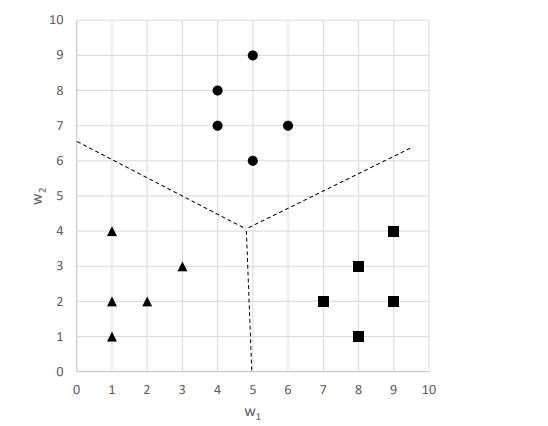
\includegraphics[width=0.8\textwidth]{chapter/chapter12/figure12_4.png}
\captionsetup{labelformat=empty}
\caption{\textbf{Figure 12.4:} Voronoi boundaries for a clustering solution of the k -means algorithm partitioning objects into three clusters.}
\label{fig12.4}
\end{center}
\end{figure}

each pair of the vertices, have their weight equal to the similarity of the corresponding documents [\cite{ref46}]. Another possibility is to represent the document set by a bipartite graph where the set of vertices consists of two sets, a set of documents and a set of terms. When a document $d_{i}$ contains a term $t_{j}$, an edge exists between these two vertices. Its weight is given by the tf-idf value of term $t_{j}$ in document $d_{i}$[\cite{ref291}].

The task of clustering documents in this representation is based on the same idea as in the case of other methods. The graph is partitioned into subgraphs so the weights of the links within clusters are high and the weights of the links between clusters are low.

\section{Clustering Criterion Functions}
During clustering, the best division of documents to clusters should be found. The quality of clustering can be measured by the function known as criterion function [\cite{ref292},\cite{ref9}] or clustering quality function [\cite{ref87}]. Clustering can be thought of as an optimization problem because it tries to find a solution that maximizes\\
or minimizes the value of the criterion function. For example, the function to be optimized (minimized) by the k -means algorithm is


\begin{equation*}
C F_{k-\text { means }}=\sum_{i=1}^{k} \sum_{d \in C_{i}} \text { similarity }\left(d, c_{i}\right), \tag{12.14}
\end{equation*}


where $k$ is the number of clusters and $c_{i}$ is the centroid of cluster $C_{i}$.\\
In some situations, the clustering criterion function is not needed because it is not feasible to evaluate all possible clustering solutions (for partitioning $n$ objects into $k$ clusters, $k^{n} / n!$ solutions would need to be examined). The algorithms are often greedy in nature and believe that using only a similarity measure to determine how much a document is similar to the objects in a cluster and dissimilar to documents in other clusters is enough [\cite{ref87}].

Various clustering criterion functions were proposed, for example, by Zhao and Karypis [\cite{ref291}]. Some of their functions are mentioned below (another set of criterion functions is presented by [9]). The functions were initially intended for partitioning algorithms but they can be used for hierarchical clustering as well. For example, instead of considering some typical merging criteria used during agglomerative clustering (see below), two clusters are merged so that the value of the criterion function improves the most. The criterion function is thus optimized only locally in a given stage of the algorithm [\cite{ref292}].

\subsection{Internal Criterion Functions}
Internal criterion functions try to maximize the similarity of documents in individual clusters while documents in different clusters are not considered. The internal criterion function $I_{1}$ maximizes the sum of average pairwise similarities between the documents assigned to each cluster, weighted according to the size of each cluster. When the cosine similarity measure is used, the $I_{1}$ function is defined as follows:


\begin{equation*}
I_{1}=\sum_{c=1}^{k} n_{c}\left(\frac{1}{n_{c}^{2}} \sum_{x_{i}, x_{j} \in C_{c}} d_{\text {cosine }}\left(x_{i}, x_{j}\right)\right), \tag{12.15}
\end{equation*}


where $k$ is the number of clusters and $n_{c}$ the number of documents in cluster $C_{c}$.

The internal criterion function $I_{2}$ maximizes the similarity between individual documents and the centroids $C_{c}$ of the clusters where the documents are assigned. The value of $I_{2}$ for the cosine similarity is calculated as


\begin{equation*}
I_{2}=\sum_{c=1}^{k} \sum_{x_{i} \in C_{c}} d_{\text {cosine }}\left(x_{i}, c_{c}\right), \tag{12.16}
\end{equation*}


where $k$ is the number of clusters and $c_{c}$ is the centroid of cluster $C_{c}$.

\subsection{External Criterion Function}
External criterion function $E_{1}$ focuses on optimization of dissimilarity of individual clusters. Thus, using this function, the documents of each cluster are separated from the entire collection:


\begin{equation*}
E_{1}=\sum_{c=1}^{k} n_{c} \cos \left(c_{c}, c_{\text {all }}\right), \tag{12.17}
\end{equation*}


where $k$ is the number of clusters, and $c_{c}$ is the centroid of cluster $C_{c}$, and $c_{\text {all }}$ is the centroid of the entire document collection. The value of $E_{1}$ is being minimized, which means that the angle of vectors $c_{c}$ and $c_{\text {all }}$ is the biggest possible.

\subsection{Hybrid Criterion Functions}
Hybrid criterion functions do not optimize only one criterion but a number of them. Instead of focusing only on intra-cluster similarity of the clustering solution while not taking into account documents in different clusters or focusing only on inter-cluster similarity and not considering similarity inside the clusters, hybrid functions combine both internal and external criteria. The two hybrid criterion functions combine the external function $E_{1}$ with $I_{1}$ or $I_{2}$ respectively:


\begin{align*}
H_{1} & =\frac{I_{1}}{E_{1}}  \tag{12.18}\\
H_{2} & =\frac{I_{2}}{E_{1}} \tag{12.19}
\end{align*}


Both internal functions $I_{1}$ and $I_{2}$ are normally maximized when the cosine similarity is used as the similarity measure. Although $E_{1}$ is normally minimized, hybrid functions $H_{1}$ and $H_{2}$ are maximized because their values are inversely related to $E_{1}$.

\subsection{Graph Based Criterion Functions}
A natural approach to graph-based clustering would be to find the minimal cut on the edges of the similarity graph $S$ (a graph where the vertices are the documents, there are edges between each pair of vertices, and the weights of the edges represent the similarity of the documents).

The edge-cut is defined as the sum of the edges connecting vertices representing documents from one cluster to vertices representing documents in other clusters:


\begin{equation*}
\sum_{c=1}^{k} \operatorname{cut}\left(S_{c}, S-S_{c}\right), \tag{12.20}
\end{equation*}


where $S$ is a similarity graph representing a document collection, $S_{c}$ is a subgraph representing cluster $c$, and $k$ is the number of clusters. Criterion function $G_{1}$, however, also considers the sum of the internal edges so it is not only the external perspective which is employed on clusters [\cite{ref73}]:


\begin{equation*}
\sum_{c=1}^{k} \frac{\operatorname{cut}\left(S_{c}, S-S_{c}\right)}{\sum_{x_{i}, x_{j} \in S_{c}} \operatorname{similarity}\left(x_{i}, x_{j}\right)}, \tag{12.21}
\end{equation*}


When the cosine similarity measure is used, the $G_{1}$ criterion function is defined as


\begin{equation*}
G_{1}=\sum_{c=1}^{k} \frac{\sum_{x_{i} \in S_{c}, x_{j} \in S-S_{c}} \cos \left(x_{i}, x_{j}\right)}{\sum_{x_{i}, x_{j} \in S_{c}} \cos \left(x_{i}, x_{j}\right)} \tag{12.22}
\end{equation*}


Since both internal and external similarities are considered in this process, this criterion function $G_{1}$ might also be perceived as a hybrid one.

The normalized cut criterion function working on a bipartite graph (vertices represent documents and terms, edges correspond to the presence of terms in the documents) looks for an optimal edge-cut. The normalized cut [\cite{ref289}] criterion function is defined as


\begin{equation*}
G_{2}=\sum_{c=1}^{k} \frac{\operatorname{cut}\left(V_{c}, V-V_{c}\right)}{W\left(V_{c}\right)}, \tag{12.23}
\end{equation*}


where $V_{c}$ is the set of vertices assigned to the $c_{t h}$ cluster, and $W\left(V_{c}\right)$ is the sum of the weights of the adjacency lists of the vertices assigned to the $c^{\text {th }}$ cluster ( $c^{\text {th }}$ cluster contains both documents as well as terms).

\section{Deciding on the Number of Clusters}
The desired number of clusters is an important parameter, especially of flat clustering algorithms. The problem is that this number is not often known in advance because the true cluster structure is unclear. In the ideal case, only a human expert can say whether a clustering solution is suitable for a specific task. Sometimes, the number of clusters might be given by technological limitations, as in the case of the Scatter-Gather algorithm, where no more than 10 clusters could originally fit to a PC screen [\cite{ref185}].

There are five clearly visible clusters on Figure 12.6. The objects were clustered to 1 to 10 clusters using the k-means method using the Euclidean distance as the similarity measure. The within cluster sum of squared errors which is minimized during clustering was calculated for each of the solutions. How the value of this measure changes depending on the number of clusters can be seen in the

\begin{figure}[H]
\begin{center}
  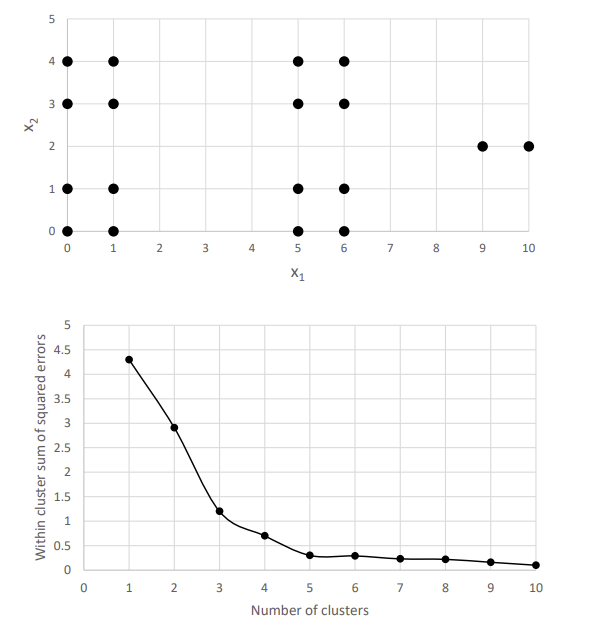
\includegraphics[width=0.8\textwidth]{chapter/chapter12/figure12_5.png}
\captionsetup{labelformat=empty}
\caption{\textbf{Figure 12.5:} A demonstration of the elbow method to determine the number of clusters. Top: Objects to be clustered. Bottom: A dependency of clustering quality on the number of clusters. A clear 'elbow' is visible at 5 clusters; from this point, no significant improvement of the clustering quality occurs.}
\label{fig12.5}
\end{center}
\end{figure}

lower part of Figure 12.6. When each object is in a separate cluster, the sum of errors is zero, which is the global minimum. The clustering, however, is not useful.

We can see that, while the value of the error function decreases quite significantly, this sharp decrease stops when the number of clusters is five. From this point, the error decreases only slightly. We can see an 'elbow' or a 'knee' on the curve approximating these values of the error. We can see that five clusters is a good compromise between the quality of clustering and the generality. Adding\\[0pt]
more clusters will not improve the solution considerably; having a smaller number of clusters, on the other hand, will increase the error significantly [\cite{ref229}]. Similarly to the within cluster sum of squared errors, any other function measuring the quality clustering can be used.

Because the goal of clustering is to discover some natural division of data, it is expected that the objects are well located within clusters and separated from the other clusters. Different clustering solutions contain groups of objects with different levels of homogeneity and separation. A measure that is able to quantify both aspects can be used as the basis for selecting the right number of clusters too. For example, the Silhouette method (see below) is one of them. The average silhouette is calculated for different clustering solutions and a solution with the best value is chosen.

There are also other recommendations depending on a specific task. For example, in information retrieval, a formula to determine the right number of clusters was developed by Can and Ozkarahan [\cite{ref42}]:


\begin{equation*}
k=\frac{m \cdot n}{t}, \tag{12.24}
\end{equation*}


where $n$ is the number of terms, $m$ the number of documents, $t$ is the total number of term assignments.

\section{K-Means}

$K$-means is the most famous algorithm for flat clustering. It iteratively improves an initial clustering solution to minimize the distance between documents and centers (means) of the clusters where the documents belong by changing cluster assignments. The procedure can be described by the following steps:

\begin{enumerate}
  \item $K$ documents (a seed) are initially selected as cluster centers $c_{1}, c_{2}, \cdots, c_{k}$.
  \item For each document $d_{i} \in D$, its nearest center $c_{j}$ is found and the document is assigned to the corresponding cluster $C_{j}\left(C_{j} \leftarrow C_{j}+\left\{d_{i}\right\}\right)$.
  \item The cluster centers are recomputed according to the current document assignment in clusters.
  \item If a stopping criterion is not met, step 2 is revisited, otherwise a clustering solution is found.
\end{enumerate}

There are a few commonly employed stopping criteria [\cite{ref185}]:

\begin{itemize}
  \item The assignment of documents to clusters (i.e., the positions of centroids) does not change between iterations. This means that a global or local optimum has been found.
  \item The value of the criterion function reaches a certain threshold. This means that the clustering solution has a sufficient quality.
  \item The change (improvement) of the the criterion function value is below a certain threshold. This means that the clustering solution almost converged to an optimal solution (maybe to a local optimum).
  \item A certain number of iterations have been carried out. This approach does not ensure that the number of iterations is sufficient to have a clustering solution of a desired quality.
\end{itemize}

If an outlier is selected as a seed it is very likely that this document will remain alone in a cluster, so it is quite useless. Removing outliers might be a good method to prevent this problem.

Selection of a suitable seed is crucial for the success of flat clustering methods because different seeds might lead to different partitionings. Thus, the algorithm can be carried out several times with a different seed and the best solution can be chosen. Alternatively, the seed can be selected based on some external knowledge as a result of hierarchical clustering method, for example [\cite{ref257}].

K-means produces convex (spherical) clusters and is not able to find clusters of other shapes. This might be a problem, especially when the clusters lie close to each other. This relates to another potential problem. The spherical shape of the produced clusters causes the cluster center to be shifted towards outliers, especially the ones placed very far [\cite{ref8}]. To overcome the sensitivity to outliers, the k-medians [\cite{ref5}] method, that uses medians instead of means for cluster representatives, can be applied.

\section{K-Medoids}
The $k$-medoids algorithm [\cite{ref7}] works in a similar fashion as the k -means algorithm. A medoid is a document that is closest to the centroid. The benefit of using the medoids instead of the means is in the decrease of computational complexity. In order to compute a distance between two documents, all non zero elements of their vectors are used in the calculation. Compared to single documents that are usually represented by very sparse vectors, centroids in the form of the cluster means contain fewer non zero elements because they average the weights of all elements of the documents in the cluster they represent. Using the medoids instead of centroids thus decreases the number of calculations when calculating the distances.

\section{Criterion Function Optimization}
Zhao and Karypis [\cite{ref294}] proposed a procedure that can be successfully used when clustering large data sets of documents. It contains an initial clustering and several iterations of cluster refinement. The goal of the refinement phase is to improve the value of a given criterion function (this algorithm may be used directly for functions $I 1, I 2, E 1, H 1, H 2$, and $G 1$; in the case of function $G 2$, the algorithm is modified so that not only vertices representing documents, but also vertices representing terms are processed). The procedure can be expressed by the following steps:

\begin{enumerate}
  \item Initially, $k$ documents are selected as the seeds.
  \item Each document is assigned to a cluster according to the most similar document from the seed.
  \item For each document (documents are visited in a random order), the following steps are carried out:
\end{enumerate}

\begin{itemize}
  \item The value of the criterion function to be optimized is calculated.
  \item The document is assigned to all other clusters and the value of the criterion function is calculated for each such assignment.
  \item The document is moved to the cluster that improves the value of the criterion function the most. It is possible that the document remains in the same cluster when no improvement can be achieved.
\end{itemize}

\begin{enumerate}
  \setcounter{enumi}{3}
  \item If some documents have been moved, step 3 is repeated, otherwise end.
\end{enumerate}

Compared to the k -means method, this method moves an object immediately after is it clear that it will improve the value of the criterion function. This is known as an incremental algorithm [\cite{ref294}].

As in the case of the k-means algorithm, this greedy approach does not have to lead to an optimal solution and a local optimum of the criterion function can be found. To prevent this, the procedure can be repeated several times and the best solution is selected.

\section{Agglomerative Hierarchical Clustering}

In agglomerative hierarchical clustering, individual documents are repeatedly merged to form larger and larger clusters. This computationally demanding procedure has the following general steps:

\begin{enumerate}
  \item All $n$ documents to be clustered are put to separate clusters (we therefore have $n$ clusters $C_{1}, C_{2}, \cdots, C_{n}$ ).
  \item The similarity of each cluster to the remaining clusters is calculated. The similarities may be contained in a similarity matrix.
  \item The maximal similarity is found so the two most similar clusters $C_{i}$ and $C_{j}$ can be identified.
  \item Clusters $C_{i}$ and $C_{j}$ are merged, so they form a new cluster.
  \item Steps 2, 3, and 4 are repeated until only one cluster remains.
\end{enumerate}

A crucial aspect of the procedure which influences the nature of created clusters, is the measure of calculating the similarity between clusters. The similarity might be based on comparing one document from each cluster, cluster centers, or all possible pairs of documents from each cluster. All of the measures use some function $d$ (e.g., the cosine similarity) to calculate a specific value of similarity of two clusters to be subsequently merged. Commonly used methods for merging clusters follow [\cite{ref5}, \cite{ref185}, \cite{ref230}, \cite{ref128}, \cite{ref45}, \cite{ref81}]:

\begin{itemize}
  \item Single Linkage Clustering (SLINK): the clusters are merged according to the similarity of the most similar objects from the clusters. It emphasizes the regions where clusters are close, ignoring the overall shape of the original and newly created clusters. Another disadvantage is the sensitivity to outliers.
\end{itemize}


\begin{equation*}
d_{\text {SLINK }}\left(H_{i}, H_{j}\right)=\min _{x_{i} \in H_{i}, x_{j} \in H_{j}} d\left(x_{i}, x_{j}\right) \tag{12.25}
\end{equation*}


When the newly created cluster is to be merged with a third cluster, the similarity can be calculated as follows:


\begin{equation*}
d_{\text {SLINK }}\left(H_{k},\left(H_{i}, H_{j}\right)\right)=\min \left(d\left(H_{k}, H_{i}\right), d\left(H_{k}, H_{j}\right)\right) \tag{12.26}
\end{equation*}


\begin{itemize}
  \item Complete Linkage Clustering (CLINK): determines the similarity according to the similarity of two most dissimilar objects. In other words, the union of two clusters has the smallest diameter and the clusters tend to be more compact. Outliers again cause the problem - here the resulting cluster will be very big.
\end{itemize}


\begin{equation*}
d_{C L I N K}\left(H_{i}, H_{j}\right)=\max _{x_{i} \in H_{i}, x_{j} \in H_{j}} d\left(x_{i}, x_{j}\right) \tag{12.27}
\end{equation*}


When merging the new cluster with another one, the distance is calculated as:


\begin{equation*}
d_{\text {CLINK }}\left(H_{k},\left(H_{i}, H_{j}\right)\right)=\max \left(d\left(H_{k}, H_{i}\right), d\left(H_{k}, H_{j}\right)\right) \tag{12.28}
\end{equation*}


\begin{itemize}
  \item Arithmetic average methods: These methods calculate the distance between two clusters to be merged as an average distance between all cluster members. The Unweighted Arithmetic Average Clustering or Unweighted Pair-Group Method using Arithmetic averages (UPGMA) gives the same weight to all objects in the computation.
\end{itemize}


\begin{equation*}
d_{U P G M A}\left(H_{i}, H_{j}\right)=\frac{1}{N_{i} \cdot N_{j}} \sum_{x_{i} \in H_{i}} \sum_{x_{j} \in H_{j}} d\left(x_{i}, x_{j}\right) \tag{12.29}
\end{equation*}


When $H_{i}$ and $H_{j}$ are merged, the distance to a third cluster, $H_{l}$ can be calculated as follows:


\begin{equation*}
d_{U P G M A}\left(H_{k},\left(H_{i}, H_{j}\right)\right)=\frac{1}{2}\left(d\left(H_{k}, H_{i}\right)+d\left(H_{k}, H_{j}\right)\right) \tag{12.30}
\end{equation*}


Information about the sizes of merged clusters is thus lost. In the Weighted Pair-Group Method using Arithmetic averages (WPGMA), the distances are weighted according to the number of objects in each cluster (bigger clusters are down-weighted):


\begin{equation*}
d_{W P G M A}\left(H_{k},\left(H_{i}, H_{j}\right)\right)=\frac{N_{i}}{N_{i}+N_{k}} d\left(H_{k}, H_{i}\right)+\frac{N_{j}}{N_{j}+N_{k}} d\left(H_{k}, H_{j}\right) \tag{12.31}
\end{equation*}


\begin{itemize}
  \item Centroid Agglomerative Clustering: This method eliminates the computational complexity of the Group Average Agglomerative Clustering method because every cluster is represented by its mean and not by all objects. When replacing all objects by their mean (centroid), the monotonicity of the combination function can be violated leading to non-intuitive dendrograms (similarity of merged clusters is higher than similarity of some previously merged clusters). It is not necessary that this approach will work well for all data sets, but is is quite successful in document clustering.
\end{itemize}

The first method, known as Unweighted Pair Group Method using Centroids (UPGMC) treats all clusters as equally important, without considering their size:


\begin{equation*}
d_{U P G M C}\left(H_{i}, H_{j}\right)=d\left(c_{i}, c_{j}\right), \tag{12.32}
\end{equation*}


where $c_{i}$ and $c_{j}$ are the centroids of clusters $H_{i}$ and $H_{j}$.

When measuring the similarity to a third cluster, the following calculation is performed:


\begin{align*}
d_{U P G M C}\left(H_{k},\left(H_{i}, H_{j}\right)\right)= & \frac{N_{i}}{N_{i}+N_{j}} d\left(H_{k}, H_{i}\right) \\
& +\frac{N_{j}}{N_{i}+N_{j}} d\left(H_{k}, H_{j}\right)  \tag{12.33}\\
& -\frac{N_{i} N_{j}}{\left(N_{i}+N_{j}\right)^{2}} d\left(H_{i}, H_{j}\right)
\end{align*}


In contrast, the Weighted Pair Group Method with Centroid (WPGMC), also known as median clustering, down-weights bigger clusters so the similarity is calculated independently of the number of objects in the clusters:


\begin{equation*}
d_{W P G M C}\left(H_{k},\left(H_{i}, H_{j}\right)\right)=\frac{d\left(H_{k}, H_{i}\right)+d\left(H_{k}, H_{j}\right)}{2}-\frac{d\left(H_{i}, H_{j}\right)}{4} \tag{12.34}
\end{equation*}


\begin{itemize}
  \item Ward Distance: Ward distance is defined as the change in the sum of squared errors of a clustering solution when two clusters are merged. The errors are calculated as a squared distance of an element from its corresponding centroid. This measure is, in fact, the value that is minimized by the k -means algorithm.
\end{itemize}


\begin{align*}
d_{\text {Ward }}\left(H_{1}, H_{2}\right) & =\sum_{x \in H_{1} \cup H_{2}}\|x-c\|^{2}-\sum_{x \in H_{1}}\left\|x-c_{1}\right\|^{2}-\sum_{x \in H_{2}}\left\|x-c_{2}\right\|^{2} \\
& =\frac{N_{1} \cdot N_{2}}{N_{1}+N_{2}} \cdot\left\|c_{1}-c_{2}\right\|^{2} \tag{12.35}
\end{align*}


where $N_{i}$ is the number of documents in cluster $i, c_{i}$ is the centroid of cluster $i$, and $c$ is the centroid of a cluster that is the union of the merged clusters [\cite{ref198}].

To generalize the calculation of the distance calculation between cluster $k$ and a cluster that was created by merging clusters $i$ and $j$, the Lance and Williams recurrence formula [\cite{ref81}] can be used:


\begin{equation*}
d_{k(i j)}=\alpha_{i} d_{k i}+\alpha_{j} d_{k j}+\beta d_{i j}+\gamma\left|d_{k i}-d_{k j}\right| \tag{12.36}
\end{equation*}


The values of parameters for the above mentioned methods can be found in Table 12.1.

\begin{table}[h]
\begin{center}
\captionsetup{labelformat=empty}
\caption{\textbf{Table 12.1:} Parameters for the Lance and Williams recurrence formula [\cite{ref81}, \cite{ref246}].}
\begin{tabular}{lccc}
\hline
Method & $\alpha_{i}$ & $\beta$ & $\gamma$ \\
\hline
SLINK & $\frac{1}{2}$ & 0 & $-\frac{1}{2}$ \\
CLINK & $\frac{1}{2}$ & 0 & $\frac{1}{2}$ \\
UPGMA & $\frac{N_{i}}{N_{i}+N_{j}}$ & 0 & 0 \\
WPGMA & $\frac{1}{2}$ & 0 & 0 \\
UPGMC & $\frac{N_{i}}{N_{i}+N_{j}}$ & $-\frac{N_{i} N_{j}}{\left(N_{i}+N_{j}\right)^{2}}$ & 0 \\
WPGMC & $\frac{1}{2}$ & $-\frac{1}{4}$ & 0 \\
Ward's & $\frac{N_{k}+N_{i}}{N_{k}+N_{i}+N_{j}}$ & $-\frac{N_{k}}{N_{k}+N_{i}+N_{j}}$ & 0 \\
Flexible $^{1}$ & $\frac{1}{2}(1-\beta)$ & $\beta<1$ & 0 \\
\hline
${ }^{1} \alpha_{1}+\alpha_{2}+\beta=1$
\end{tabular}
\end{center}
\label{table12.1}
\end{table}

\section{Scatter-Gather Algorithm}
Flat methods are more efficient compared to the hierarchical methods. They are, however, dependent on the initial seed (e.g., initial cluster centers in the k-means method) so they are not as robust as the hierarchical algorithms that compare all pairs of documents. A solution is to combine both approaches to a hybrid method used in the Scatter-Gather algorithm. The Scater-Gather method is originally a document browsing method that partitions (scatters) a document collection to a small number of groups and presents their short summaries to a user. One or more groups are selected (gathered) by the user and these groups are further analyzed using the same approach (i.e., clustering, summary, and groups selection). By a repeated application of these scatter and gather steps, the gathered clusters are more and more detailed and closer to the user's information need [\cite{ref61}].

Such an approach requires a fast clustering phase so a hybrid approach using a hierarchical method to select $k$ seeds to be used in a flat method was proposed in [\cite{ref61}]. To select the initial seed, two approaches might be used:

\begin{itemize}
  \item Buckshot: Having $n$ documents to be clustered into $k$ clusters, $\sqrt{k \cdot n}$ documents are randomly selected and clustered using an agglomerative method to form $k$ clusters. These $k$ clusters then become the seeds for a flat method applied to the entire data set. Because the complexity of a hierarchical method is $O\left(n^{2}\right)$, using only about the square root of the documents, the complexity becomes $O(k \cdot n)$.
  \item Fractionation: The documents are divided into $n / m$ buckets where $m>k$ is the size of each bucket. In each bucket, the documents are clustered using an agglomerative hierarchical method until the number of clusters in a bucket is reduced by a certain factor (initially, the number of clusters
\end{itemize}

\begin{figure}[H]
\begin{center}
  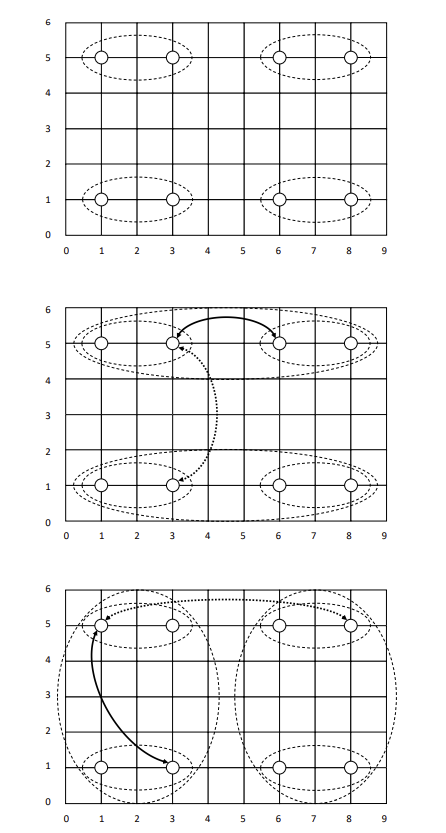
\includegraphics[width=0.5\textwidth]{chapter/chapter12/figure12_6.png}
\captionsetup{labelformat=empty}
\caption{\textbf{Figure 12.6:} A demonstration of the difference between SLINK and CLINK methods. Top: An initial clustering solution. Middle: Newly created clusters using SLINK. The distance between the most similar objects represented by the solid line is smaller than the one represented by the dotted line. Bottom: Newly created clusters using CLINK. The distance between the most dissimilar objects represented by the solid line is smaller than the one represented by the dotted line.}
\label{fig12.6}
\end{center}
\end{figure}

\hspace{-1.5em}is equal to the number of documents in a bucket). Subsequently, the process of rearranging the objects (documents or clusters of documents) into buckets and agglomerating them is repeated until there are $k$ seeds (roots of dendrograms obtained by the agglomeration procedure) found.\\
To further improve the seed selection results, the documents are not assigned to the buckets completely randomly, but they are first ordered according to the value of the index of the $i^{\text {th }}$ most frequent word in each document ( $i$ is typically a smaller number, such as three, so medium frequency words are favoured). This ensures that documents that are close in this ordering share at least one word.

To increase the speed of computation of the buckshot phase, Liu et al. [\cite{ref180}] use the initial $k$ centroids that are found in a pre-computed hierarchical agglomeration structure constructed in the first phase of their algorithm

\section{Divisive Hierarchical Clustering}
Divisive clustering constructs the hierarchy in a top-down manner. All documents are initially in one cluster which is recursively divided until we have only singleton clusters. To obtain the same type of hierarchy as in case of agglomerative clustering, the cluster is usually divided into two sets.

The procedure of divisive clustering has the following general steps:

\begin{enumerate}
  \item All $n$ documents to be clustered are put to one cluster.
  \item The cluster is partitioned to $m$ clusters, usually using a flat method.
  \item Step 2 is recursively applied to newly created clusters until every document is in a separate cluster.
\end{enumerate}

The problem of divisive clustering is that having $n$ documents, they can be split into $2^{n-1}-1$ possible non-empty groups. Even for a low $n$ there are so many possibilities that it is not computationally feasible to choose the best split [\cite{ref285}].

In divisive clustering, is is often not necessary to build a complete dendrogram. At times, it may be useful to set some termination criteria for splitting the clusters to get a meaningful result, also because the clustered data can contain noise. Thus, particularly when no complete hierarchy needs to be created, the divisive clustering procedure is more efficient than the agglomerative [\cite{ref222}]. The stopping criteria may include [\cite{ref53}]:

\begin{itemize}
  \item $k$ clusters are found,
  \item maximal hierarchy depth is reached,
  \item minimum number of documents in a cluster remain,
  \item minimal desired homogeneity (dissimilarity) in a cluster is achieved.
\end{itemize}

To get a hierarchy of clusters, a flat method is often recursively applied to the clusters being created. The flat methods that are usually used to split a cluster into more clusters require a number of clusters as an input. Thus, splitting a cluster into two (bi-partitioning) is a common approach. In this way, the created hierarchical structure has the same form as the one created in an agglomerative procedure when two clusters are merged [\cite{ref53}]. If the same type of dendrogram that is a result of an agglomerative method is to be obtained, a sequence of $n-1$ ( $n$ is the number of documents) bisections should be applied to the data (bisection means splitting a set into two subsets) [\cite{ref293}].

Other possibilities of creating a cluster hierarchy include trying all possibilities of splits and evaluating them using the same metrics as in the case of agglomerative methods [232, 55]. However, because complete information about all objects is initially available, such divisive clustering can be considered to be a global approach [\cite{ref222}] unlike agglomerative clustering.

In the divisive approach, the question is, which of the clusters to split. There are a few possible approaches [\cite{ref294}, \cite{ref240}]:

\begin{itemize}
  \item In the simplest approach, the larger cluster is divided. In many cases, this leads to reasonably good and balanced clustering solutions. However, this approach is not suitable when naturally large clusters exist, because these large clusters will be divided first.
  \item One of the current clusters is split so the value of a selected criterion function improves the most. Often, the cluster with the largest variance (i.e., the average squared distance to the cluster centroid) is selected, which is in fact optimization of the internal criterion function.
\end{itemize}

An example of the divisive clustering method is the bisecting k-means algorithm. The documents forming one cluster are split into two clusters using the basic k-means algorithm. Then, the cluster with a higher number of objects or with the largest variance is selected and split again. The selection and splitting steps are repeated until a desired number of clusters is reached or when a complete hierarchy is created [\cite{ref256}]. It has been found in the text mining domain, that the bisecting k-means is generally better for higher numbers of clusters than the direct k-means method [\cite{ref141}, \cite{ref294}].

\section{Constrained Clustering}
Agglomerative hierarchical clustering is strictly local and does not take the properties of the entire data set into consideration. This might be a disadvantage in
some situations, especially when clustering documents share a large portion of their vocabulary. To prevent such a problem, an agglomerative clustering procedure using constraints imposed by a flat clustering is an option. Initially, the entire collection is partitioned to $k$ constraint clusters and clustering then takes place only within these clusters. It is, therefore, not possible to merge documents or clusters from different constraint clusters. This approach combines the global view of flat methods and local view of agglomerative methods. The time complexity of the agglomerative algorithm is also decreased [294].

Another possibility of change in the unsupervised process of clustering is to bring some external knowledge in the form of must-links (information about objects that must be in the same cluster) and cannot-links (information about objects that cannot be in the same cluster) [\cite{ref18}]. The COP-K-means algorithm proposed by [\cite{ref272}] then simply modifies the steps of the traditional k-means algorithm:

\begin{enumerate}
  \item $K$ documents (a seed) are initially selected as cluster centers $c_{1}, c_{2}, \cdots, c_{k}$.
  \item For each document $d_{i} \in D$, its nearest center $c_{j}$ that does not violate any constraint is found. Subsequently, the document is assigned to the corresponding cluster $C_{j}\left(C_{j} \leftarrow C_{j}+\left\{d_{i}\right\}\right)$. If no cluster satisfying the constraints is found, the procedure fails.
  \item According to the current document assignment in clusters, the cluster centers are recomputed.
  \item If a stopping criterion is not met, go to step 2 , otherwise a clustering solution is found.
\end{enumerate}

\section{Evaluating Clustering Results}
The general goal of clustering is to find some interesting structure in data. As there is usually no prior knowledge about the desired outcome and several alternative results are possible, evaluating clustering is not an easy task. Clustering also should not be considered an isolated mathematical problem but should always be studied in the context of a given task where it is employed [\cite{ref268}, \cite{ref115}]. Besides using some mathematical computations described in this section, the suitability or usefulness of clustering for a specific application can be measured very naturally. For example, [\cite{ref185}] use the time needed to find a desired answer in an information retrieval task that used clustering to navigate search results.

The goal of clustering evaluation is often to compare different clustering experiments and results. It is therefore desirable to use a simple numeric measure that is not biased toward a specific number and sizes of clusters and similarity measures, one that can easily be interpreted and can be used for a single cluster as well as for the entire clustering solution [\cite{ref244}].

Internal (or intrinsic) measures evaluate clustering based solely on the information contained in the data. They usually depend on the representation of data (choice of features) and cannot be compared for different representations. External (or extrinsic) evaluation measures use some kind of external knowledge. This can be the existence of known classes (ground truth labelling) or the relevance judgements of human experts [\cite{ref68}, \cite{ref127}].

Internal measures can give us information about how similar the generated clusters are inside (cohesion), how distinct from other clusters (separation), or both. Obviously, having only singleton clusters will lead to a situation where perfect homogeneity within clusters is achieved. Having only one cluster means that the dissimilarity with other clusters reaches a zero level. Both situations are thus optimal from one of the perspectives. However, since these two possibilities often do not match the reality, they are not desirable [\cite{ref244}]; the number of clusters should be low [\cite{ref115}] and some compromise needs to be found. The above mentioned clustering criterion functions can serve as internal measures of clustering quality. Another well known method is the silhouette method.

For external cluster evaluation, some kind of human judgement is often needed. The problem is that human judgements can be very subjective because everyone can have a different opinion about the topic. A correct answer to a clustering problem is also often not available. External evaluation looks at the closeness to a clustering provided by a human. Human experts thus usually create clusters that are compared to the clusters generated by an algorithm. Typical measures include purity, entropy, normalized mutual information, or F-measure.

The assignment of objects to clusters in the calculated clustering $U$ and the real (or expected) clustering $V$ can often be expressed in the form of a contingency table; see Figure 12.7. In the solution $U$, there exist $R$ clusters, $S$ clusters are defined in the $V$ clustering. The value on the $\mathrm{i}^{\text {th }}$ row and $\mathrm{j}^{\text {th }}$ column denotes the number of objects belonging to clusters $U_{i}$ and $V_{j}$ [\cite{ref267}]. We can say that for these objects, the found and real assignment to a cluster agree. Based on the numbers from the contingency table, the values of some external cluster validity measures can be calculated.

\begin{table}[h]
\begin{center}
\begin{tabular}{l|llll}
 & $V_{1}$ & $V_{2}$ & $\cdots$ & $V_{S}$ \\
\hline
$U_{1}$ & $n_{11}$ & $n_{12}$ & $\cdots$ & $n_{1 S}$ \\
$U_{2}$ & $n_{21}$ & $n_{22}$ & $\cdots$ & $n_{2 S}$ \\
$\vdots$ & $\vdots$ & $\vdots$ & $\ddots$ & $\vdots$ \\
$U_{R}$ & $n_{R 1}$ & $n_{R 2}$ & $\cdots$ & $n_{R S}$ \\
\end{tabular}
\captionsetup{labelformat=empty}
\caption{\textbf{Figure 12.7:} A contingency table characterizing an agreement between two clustering solutions, $U$ and $V$.}
\end{center}
\end{table}

When evaluating clustering, compactness inside the clusters and separation of clusters are usually considered. Other factors, such as geometric or statistical properties of the data, the number of data objects, and dissimilarity or similarity measurements can be considered too [\cite{ref45}]. Besides satisfying the homogeneity and separation criteria, clusters should also be complete. This means that objects from one class should be placed to one cluster. Another desirable property of clustering is to assign items not belonging to classes that are contained in clusters to a separate cluster. This cluster, containing 'other' or 'miscellaneous' elements, does not introduce disorder to existing clusters [\cite{ref13}].

\subsection{Metrics Based on Counting Pairs}
One possibility of evaluating clusters is to calculate the statistics based on looking at how pairs of objects are placed to clusters in a clustering solution and a predefined partition [13]. Let there be $n$ objects $x_{1}, \ldots, x_{n}$ clustered to clusters $C_{1}$, $\ldots, C_{k}$. In addition, we have a defined partition (ground truth) $P_{1}, \ldots, P_{l}$. Looking at each pair ( $x_{i}, x_{j}$ ) from the data set, the following situations can occur:

\begin{itemize}
  \item $S S$ : the objects belong to the same cluster of $C$ and to the same cluster of $P$.
  \item $S D$ : the objects belong to the same cluster of $C$ and to different clusters of $P$.
  \item DS: the objects belong to different clusters of $C$ and to the same cluster of $P$.
  \item $D D$ : the objects belong to different clusters of $C$ and to different clusters of $P$.\\
$S S+S D+D S+D D$ is the number of pairs of data which equals to $n(n-1) / 2$. $S S$ and $D D$ are good assignments, $S D$ and $D S$ are bad assignments.
\end{itemize}

The degree of similarity between a created clustering solution and the ground truth can be characterized by the following indices:


\begin{gather*}
\text { Rand Statistic }=\frac{S S+D D}{S S+S D+D S+D D}  \tag{12.37}\\
\text { Jaccard Coefficient }=\frac{S S}{S S+S D+D S}  \tag{12.38}\\
\text { Folkes and Mallows Index }=\sqrt{\frac{S S}{S S+S D} \frac{S S}{S S+D S}} \tag{12.39}
\end{gather*}


High values of these indices indicate a good match between $C$ and $P$ [\cite{ref110}].

\subsection{Purity}
Purity measures the fraction of a majority class in a cluster $C_{i}$ :


\begin{equation*}
\operatorname{Purity}\left(C_{i}\right)=\max _{j \in L} \frac{l_{i j}}{\left|C_{i}\right|}, \tag{12.40}
\end{equation*}


where $L$ is a set of classes, $l_{i j}$ is the number of documents from class $j$ in cluster $C_{i}$, and $\left|C_{i}\right|$ is the number of documents from cluster $C_{i}$. When a cluster contains instances from only one class, it is perfectly pure (clean) and the value of purity equals to 1 . Purity of the entire clustering solution can be calculated as a weighted average of purities of all clusters:


\begin{equation*}
\text { Purity }=\sum_{i=1}^{k} \frac{\left|C_{i}\right|}{n} \text { Purity }\left(C_{i}\right), \tag{12.41}
\end{equation*}


where $k$ is the number of clusters and $n$ is the number of documents in the clustering solution.


\subsection{Entropy}
Entropy is an alternative measure expressing how many clusters contain documents from one class. Entropy, as proposed by Shannon, measures the average amount of information that is received in incoming messages; see section 14.3.2. The lowest entropy (value 0 ) is achieved when only one possible outcome exists. The highest value is in the case that all outcomes are equally likely. Entropy can thus be used for measuring the quality of clusters [\cite{ref256}]. The best quality of a cluster is achieved when the cluster contains instances from one class. In this case, there are no surprises and the entropy is 0 . The highest entropy \{value $\log (c)$, where $c$ is the number of classes $\}$ and thus the worst quality of a cluster is obtained when there are instances of more than one class in the cluster and the numbers of documents from each class are equal. To calculate entropy, probabilities $p_{i j}$ that a document $j$ belongs to each of classes $j \in L$ must be calculated first:


\begin{equation*}
p_{i j}=\frac{l_{i j}}{\left|C_{i}\right|}, \tag{12.42}
\end{equation*}


where $l_{i j}$ is the number of documents from class $j$ in cluster $C_{i}$ and $\left|C_{i}\right|$ is the number of documents from cluster $C_{i}$.

Entropy of the cluster $i$ is then calculated as


\begin{equation*}
\text { Entropy }\left(C_{i}\right)=\sum_{j \in L} p_{i j} \log p_{i j} \tag{12.43}
\end{equation*}


To get the entropy of the entire clustering solution, we calculate the sum of the entropies of all clusters weighted according to their sizes:


\begin{equation*}
\text { Entropy }=\sum_{i=1}^{k} \frac{\left|C_{i}\right| \text { Entropy }\left(C_{i}\right)}{n}, \tag{12.44}
\end{equation*}


where $k$ is the number of clusters and $n$ is the number of instances to be clustered.

\subsection{F-Measure}
$F$-measure is often used in information retrieval and classification but its idea is suitable for evaluating clustering as well. It combines the values of the precision (the fraction of documents from a desired class that are placed to a cluster) and recall (the fraction of documents that should be put to a cluster and are really there). Both values are always calculated with respect to the given cluster and class. The precision for class $j$ in cluster $C_{i}$ can be calculated as


\begin{equation*}
\operatorname{Precision}(i, j)=\frac{l_{i j}}{\left|C_{i}\right|}, \tag{12.45}
\end{equation*}


where $l_{i j}$ is the number of instances of class $j$ in cluster $C_{i}$ and $\left|C_{i}\right|$ is the total number of instances in cluster $C_{i}$. The recall for class $j$ in cluster $C_{i}$ is calculated as


\begin{equation*}
\operatorname{Recall}(i, j)=\frac{l_{i j}}{l_{j}}, \tag{12.46}
\end{equation*}


where $l_{i j}$ is the number of instances of class $j$ in cluster $C_{i}$ and $l_{j}$ is the total number of documents of class $j$. The value of F -measure is typically calculated as the harmonic mean of the precision and recall:


\begin{equation*}
F(i, j)=2 \frac{\operatorname{Precision}(i, j) \operatorname{Recall}(i, j)}{\operatorname{Precision}(i, j)+\operatorname{Recall}(i, j)} \tag{12.47}
\end{equation*}


The overall F -measure for the entire clustering solution is the averaged F measure for all classes distributed over all clusters [255]:


\begin{equation*}
F=\sum_{j=1}^{l} \frac{l_{j}}{n} \max _{i=1 . . k} F(i, j) \tag{12.48}
\end{equation*}


where $l$ is the number of classes, $l_{j}$ is the number of instances from the class $j$, $n$ is the number of all instances, and $k$ is the number of clusters. To achieve high values of the F-measure, both the precision and recall need to be high. Then the value of the F -measure will be close to 1 .

\subsection{Normalized Mutual Information}
Normalized Mutual Infromation (NMI) belongs to the class of information theoretic measures. It measures how much information two clusterings, one found by an algorithm and the other created by a human, share. In other words, NMI tells us how much knowing about one of the clustering solutions reduces uncertainty about the other. Mutual information $I(U, V)$ of clusterings $U$ and $V$ is the difference between entropy of $U$ (the average amount of information needed to encode the labels of every object in $U$ ) and the entropy $H(U \mid V)$, which is the average amount of information needed to encode the labels of objects in $U$, knowing $V$ :


\begin{equation*}
I(U, V)=H(U)-H(U \mid V) \tag{12.49}
\end{equation*}


Alternatively, mutual information can be expressed as the sum of entropies of $U$ and $V$ minus the joint entropy of $U$ and $V$ :


\begin{equation*}
I(U, V)=H(U)+H(V)-H(U, V) \tag{12.50}
\end{equation*}


The entropy of $U$ can be calculated as follows:


\begin{equation*}
H(U)=-\sum_{i=1}^{k} p_{i} \log \left(p_{i}\right), \tag{12.51}
\end{equation*}


where $p_{i}$ is the probability of an object being in cluster $C_{i}$, i.e., $p_{i}=\left|C_{i}\right| / n$ ( $\left|C_{i}\right|$ is the size of cluster $C_{i}$ and $n$ is the number of all objects).


\begin{equation*}
H(U \mid V)=-\sum_{i=1}^{R} \sum_{i=1}^{S} \frac{n_{i j}}{n} \log \frac{n_{i j} / n}{n_{j} / n}, \tag{12.52}
\end{equation*}


where $R$ is the number of clusters in $U, S$ is the number of clusters in $V, n_{i j}$ the number of objects placed to the same cluster in both $U$ and $V$, and $n_{j}$ is the number of objects in cluster $V_{j}$.

The joint entropy of $U$ and $V$ can be expressed as:


\begin{equation*}
H(U, V)=-\sum_{i=1}^{R} \sum_{i=1}^{S} \frac{n_{i j}}{n} \log \frac{n_{i j}}{n} \tag{12.53}
\end{equation*}


The mutual information can be expressed by the following formula:


\begin{equation*}
I(U, V)=-\sum_{i=1}^{R} \sum_{i=1}^{S} \frac{n_{i j}}{n} \log \frac{n_{i j} / n}{n_{i} n_{j} / n^{2}}, \tag{12.54}
\end{equation*}


where $n_{i}$ is the number of objects in cluster $U_{j}$ and the meaning of the other symbols is the same as in the previous formula [\cite{ref267}, \cite{ref12}].

To be able to use mutual information for comparing different clustering solutions, a normalized version is often used. A few normalization schemes already\\
exist. $N M I(U, V)=2 I(U, V) /(H(U)+H(V))$ [\cite{ref185}] is probably the most popular normalization which scales the values of mutual information to the interval [0.1].

\subsection{Silhouette}
The silhouette method was proposed by Rousseeuw [\cite{ref231}]. It looks at every single object and calculates how well is it located in its cluster and separated from the other clusters. To construct a silhouette, any distance metric can be used.

For every object $d_{i}$ from cluster $C_{i}$, the average distance $a_{i}$ (dissimilarity) of $d_{i}$ from all other objects in $C_{i}$, is calculated. The smaller the value, the better. A small value means that the objects in a cluster are homogeneous, closer to each other.

Subsequently, similar values are calculated for $d_{i}$ and all other clusters $C_{j}, j=1 \ldots k, j \neq i$ (i.e., average distances of $c_{i}$ from objects in other clusters). The higher the value for a cluster $C_{j}$ the better it is because $d_{i}$ is different from the objects in that cluster. The minimal value $b_{i}$ from these average distances denotes the closest cluster (neighbor), i.e., the second best cluster choice for object $d_{i}$.

The silhouette for $d_{i}$ is calculated from $a_{i}$ and $b_{i}$ as follows:

\[
s(i)=\left\{\begin{array}{ll}
1-\frac{a_{i}}{b_{i}} & \text { if } a_{i}<b_{i}  \tag{12.55}\\
0 & \text { if } a_{i}=b_{i} \\
\frac{b_{i}}{a_{i}}-1 & \text { if } a_{i}>b_{i}
\end{array}\right\}=\frac{b_{i}-a_{i}}{\max \left\{a_{i}, b_{i}\right\}}
\]

From the formula, it is obvious that the value of $s(i)$ lies between -1 and 1 (both values are included). When cluster $C_{i}$ contains only one object, the value of $a_{i}$ cannot be calculated so it is usually 0 .

When the value of $s(i)$ is close to 1 , the dissimilarity inside the cluster $a_{i}$ is much lower than the dissimilarity between clusters. This means that the object is well clustered (assigned to a correct cluster) because the objects in the second best cluster are much more dissimilar.

If the value of $s(i)$ close to -1 , the object has most likely been placed to a wrong cluster; it would be better to have it in another cluster where the objects are more similar to it on average.

Value 0 indicates that the object is exactly between the best and the second best clusters and it could be put to either of them ( $a_{i}$ and $b_{i}$ are equal).

When similarities need to be used instead of dissimilarities, the formulae for calculating the value of $s(i)$ need to be modified:

\[
s(i)= \begin{cases}1-\frac{b_{i}^{\prime}}{a_{i}^{\prime}} & \text { if } a_{i}^{\prime}>b_{i}^{\prime}  \tag{12.56}\\ 0 & \text { if } a_{i}^{\prime}=b_{i}^{\prime} \\ \frac{a_{i}^{\prime}}{b_{i}^{\prime}}-1 & \text { if } a_{i}^{\prime}<b_{i}^{\prime}\end{cases}
\]

The silhouette method is based on a principle similar to the group average linkage methods so it works well for roughly spherical clusters.

A great advantage of the silhouette method is the ability to visualize the correctness of assignment of objects in clusters. A typical graphical representation is a plot where every object is depicted by one horizontal line with the size proportional to the value of $s(i)$. If the value of $s(i)$ is negative, the line is drawn in the opposite direction to the lines representing objects with positive values of $s(i)$. All lines are arranged one above the other, beginning at the same position. The objects in one cluster are in one group where the objects are sorted according to the value of $s(i)$ with the highest value first.

Intuitively, higher values of $s(i)$ are preferred to lower values. Thus, cluster 1 in Figure 12.8 is better than cluster 2 because its silhouette is wider. It is also desirable that there are no objects with low values of $s(i)$. Examples of this are the last two objects in cluster 3 where the last one should even be put to a different cluster as it is more similar to a cluster other than cluster 3.

The silhouette method can be also used to find a correct number of clusters. The silhouettes for different clustering solutions can be analyzed and the solution with the best cluster silhouettes is selected.

If the number of clusters to be created is too high, some naturally occurring clusters will be split into more clusters (in a situation where the natural clusters are very homogeneous and far from the others). For example, objects in a natural cluster A will be placed to clusters B and C. These clusters will still be quite

\begin{figure}[H]
\begin{center}
  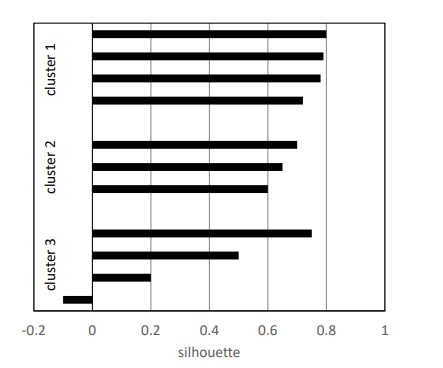
\includegraphics[width=0.7\textwidth]{chapter/chapter12/figure12_8.png}
\captionsetup{labelformat=empty}
\caption{\textbf{Figure 12.8:} An example of the silhouette values for a clustering solution of several objects into three clusters.}
\label{fig12.8}
\end{center}
\end{figure}

homogeneous but very similar to each other. Thus, the values of $s(i)$ will be rather small compared to the situation when we have only cluster A.

When the number of clusters is too low, some of the clusters that should be separated will be merged. Now, the internal similarity will be higher, which will again lead to lower values of $s(i)$.

We can also calculate an average silhouette width for each cluster. This is simply the arithmetic average of the values of $s(i)$ for all objects in cluster $C_{j}$ :


\begin{equation*}
s\left(C_{j}\right)=\frac{1}{\left|C_{j}\right|} \sum_{x \in C_{i}} s(x) \tag{12.57}
\end{equation*}


Clusters with high values of average silhouette width are more obvious than those with lower values. We can even calculate the average silhouette width for all objects in the entire data set:


\begin{equation*}
s(k)=\frac{1}{k} \sum_{r=1}^{k} s\left(C_{r}\right) \tag{12.58}
\end{equation*}


The clustering solution with the highest value [\cite{ref8}] will be preferred.

\subsection{Evaluation Based on Expert Opinion}
When no prior knowledge about the expected outcomes of clustering is available, an expert can inspect the results and decide about their usefulness. This kind of validation carried out by human experts is suitable under many circumstances. It may reveal new insights into the data, but is generally very expensive and demanding. The results, which are subjectively influenced are also not comparable.

The objects to be clustered are characterized by some attributes and their values. Each object can be thus seen as a multidimensional vector or a point in a multidimensional space where the number of dimensions is equal to the number of attributes. Intuitively, the clusters can be defined as sub-spaces containing the objects which are clearly separated from the other sub-spaces. This identification can be thus done visually by a human expert. However, the problem is when the number of dimensions is greater than three. There are methods that are able to project objects from a multidimensional space to a two- or three-dimensional space. This enables the users to examine visually whether the created clusters correspond to the clusters that they can see. Such an approach is based on the principle that groups of objects that are separated in 2D or 3D are also separated in a space with many dimensions [\cite{ref122}]. This kind of evaluation is, however, difficult to use for data with a very high number of dimensions, which is the case of textual document collections.

The experts might also examine the objects in individual clusters and consider the extent to which such an arrangement contributes to the objective of a given task. In the case that many objects are clustered, such a manual process would\\[0pt]
be very difficult and thus unfeasible. In that case it is possible to not consider all of the documents but examine only some of them. There are several approaches to choose the representative documents [\cite{ref99}]. A user might be presented with a document which is:

\begin{itemize}
  \item an average document - the document lies most closely to the remaining documents in the cluster, i.e., it is located near the centroid of the cluster;
  \item the least typical element - the document is close the border of the cluster, closer to the remaining clusters; it is most similar to documents in the other clusters;
  \item the most typical - the document is located near the border of the cluster, far from the other clusters; it is the most different from all of the documents in the collection and thus the most specific.
\end{itemize}

The documents found by using the last two approaches might be difficult to interpret, especially in the case that there are many clusters in the clustering solution. Therefore, choosing a document that is located in the center of a cluster seems to be appropriate.

Sometimes, one document may not be informative enough. Therefore, more documents selected using the same criterion might be used. In that situation, the documents can be ranked according to the given criterion and a few documents which lie at the top of such a list of ranked documents can be presented.

\section{Cluster Labeling}

Sometimes, not only are the labels for the data not assigned to the documents but the labels may not even exist. Consider a company selling some products or providing some services. On some web pages, the customers have the facility to talk about them, evaluate them, or simply send complaints electronically, everything freely written using a natural language. Reading thousands of such messages by a human expert and identifying the major topics that are mentioned would not be feasible. Instead of that, a computer might try to find groups of documents that are somehow similar and distinguished from the other groups. These groups will be more or less related to individual aspects of the product or service. Subsequently these groups might be further processed so that typical representatives of the groups or keywords characterizing the groups can be retrieved and used to, for example, improve the business quality. Such keywords are often referred to as cluster labels. It is generally good to characterize the clusters using a small number of variables [\cite{ref115}]

According to Ferraro and Wanner [\cite{ref88}], two main strategies of document cluster labeling can be identified. In internal cluster labeling, which is usually quite\\
a simple approach, the label of the cluster is based solely on the content of the cluster. The title of a representative document or a list of words that appear with a sufficiently high frequency might be used. In differential cluster labeling, the label is determined by contrasting the cluster with other clusters. When a candidate label depends on a cluster more than on the other clusters, it is considered a good label for that cluster. Several statistical measures, such as mutual information, information gain, or chi squared might be applied.

\section{A Few Examples}
The following example shows how to cluster a document set, determine a suitable number of clusters, evaluate alternative clusterings, and characterize the found clusters.

In the first example, only eight documents that were manually created are processed. Here, a reader clearly sees the content of the documents and makes decisions about assigning them to clusters. The documents, most naturally, form tree clusters:

\begin{itemize}
  \item One is about clustering:
  \item Document 1: Clustering is an unsupervised machine learning method and assigns data to groups.
  \item Document 2: Clustering finds groups in data in an unsupervised way.
  \item The other is related to classification:
  \item Document 3: Classification is a supervised machine learning method and assigns a class to an object.
  \item Document 4 : A class is determined in a supervised classification.
  \item The last one mentions statistics (the last two documents are more similar than the first two because they both mention analysis and summarization):
  \item Document 5: Statistical analysis can be applied to large data sets.
  \item Document 6: Statistics deals with large data sets analysis.
  \item Document 7: Statisticians analyze and summarize large data sets.
  \item Document 8 : It is fun to analyze and summarize data.
\end{itemize}

To be able to cluster the data, a conversion to a numerical document-term matrix is performed using the tm package.

The data is then clustered using several algorithms. Some of them work with a data matrix representing the objects to be clustered, some others accept a dissimilarity matrix containing pairwise dissimilarities of all pairs of objects. The\\
dissimilarity matrix can be calculated using the dist() function from the stats package or with the daisy() function from the cluster package.

The kmeans() function from package stats is used to cluster the data in a matrix using the k -means algorithm. The function requires a numeric matrix of data (or an object that can be coerced to such a matrix), the number of clusters to be found, or a set of initial cluster centres. If the initial centers are not provided, a random set of rows in the data matrix is chosen as the initial centres. We might also supply the maximum number of iterations of the algorithm.

The function returns an object of class kmeans. Its components include cluster - a vector of integers indicating the cluster to which each point belongs, centers - a matrix of cluster centres, or size - the number of objects in each cluster.

In our example, values 2, 3, and 4 are successively supplied as the parameters determining the number of clusters. For each clustering solution, assignment of the documents to clusters is displayed by printing the contents of the cluster element of the clustering list. Then, the silhouette() function from package cluster is used to calculate the values of the silhouette for each document. The first parameter of the function contains an object of an appropriate class, an integer vector with k different integer cluster codes or a list with such a clustering component by default. The other parameters include a dissimilarity matrix (dist), that can be in its symmetric form (dmatrix). The function returns a silhouette class object, which is an $\mathrm{n} \times 3$ matrix with attributes. Each row (document) contains the cluster to which it belongs, the neighbour cluster (the cluster not containing the document, for which the average dissimilarity is minimal), and the silhouette width (the column names are cluster, neighbor, and sil\_width). The values of silhouette can be sorted so they can be displayed in the usual way - objects from one cluster together, in a descending order.

Function sortSilhouette() orders the rows of a silhouette object increasingly by cluster and with decreasing silhouette width. To visualize the silhouette, the standard plot() function can be used. We can also use the package factoextra that provides functions that can be used to extract and visualize the results of multivariate data analyses. One of them, fviz\_silhouette(), visualizes silhouette information from clustering.

We can see that the solution with three clusters has the highest value of silhouette, significantly higher than for the solution with two clusters. The silhouette for the solution with three clusters also looks much better that the solution with two clusters. Four clusters seem to be only slightly worse than three clusters as the last four documents can be considered one or two clusters.

As the k-means method used in this example depends on some random initialization, a reader can sometimes obtain different results (typically, the documents will be differently distributed in the generated clusters).

\begin{verbatim}
library(tm)
library(ggplot2)
library(factoextra)
# converting texts to a structured representation
texts <- c("Clustering is an unsupervised machine
        learning method and assigns data to groups",
    "Clustering finds groups in data in an
            unsupervised way",
    "Classification is a supervised machine learning
        method and assigns a class to an object",
    "A class is determined in a supervised
        classification",
    "Statistical analysis can be applied to large
        data sets",
    "Statistics deals with large data sets analysis",
    "Statisticians analyze and
        summarize large data sets",
    "It is fun to analyze and summarize data.")
documents <- data.frame(doc_id=1:8,
            text=texts,
            stringsAsFactors = FALSE)
corpus <- Corpus(DataframeSource(documents))
corpus <- tm_map(corpus, removePunctuation)
corpus <- tm_map(corpus, content_transformer(tolower))
dtm <- DocumentTermMatrix(corpus,
    control = list(
    wordLengths = c(1, Inf),
    weighting=function (x) weightSMART(x,spec="ntn")
    )
)
# a matrix to be used by kmeans()
mat <- as.matrix(dtm)
# a distance matrix to be used for silhouette calculation
distances <- dist(mat)
# an object for storing silhouette values for
# different partitionings
silhouette <- matrix(0, nrow=4, ncol=8)
# trying three different partitionings
for (nclust in 2:4) {
\end{verbatim}

\begin{verbatim}
    print(paste("Number of clusters:", nclust))
    clustering <- kmeans(mat, nclust)
    # looking at assignment of document to clusters
    print("Cluster assignment:")
    print(clustering$cluster)
    # looking at most important features characterizing
    # a cluster
    for (c in 1:nclust) {
        print(paste(paste("Cluster", c), ":"))
        print(sort(clustering$centers[c,], decreasing=TRUE)[1:5])
    }
    # computing sihlouette information
    sil <- silhouette(clustering$cluster, dist=distances)
    # storing the values of silhouette for a clustering result
    silhouette[nclust, ] <- as.vector(sortSilhouette(sil)[,3])
    # plotting a silhouette graph
    plot(fviz_silhouette(sil, label=TRUE, print.summary=TRUE))
}
# printing silhouette information for different partitionings
for (nclust in 2:4) {
    print(paste("Silhouette for cluster ", nclust))
    print(round(silhouette[nclust, ], 3))
    print(paste("Mean:", round(mean(silhouette[nclust, ]), 3)))
}
\end{verbatim}

The output obtained from the executed statements gives us information on how the documents were assigned to clusters (each cluster is labeled with a number, the numbers start from 1), what features characterize them well, silhouette information, and plots with visualized silhouette information (see Figure 12.9):

\begin{lstlisting}
[1] "Number of clusters: 2"
[1] "Cluster assignment:"
1 2 3 4 5 6 7 8
1 1 1 1 2 2 2 2
[1] "Cluster 1:"
a           in          an          assigns     clustering
2.000000    1.500000    1.061278    1.000000    1.000000
[1] "Cluster 2 :"
large       sets        analysis    analyze     summarize
1.061278    1.061278    1.000000    1.000000    1.000000

cluster size ave.sil.width
1       1    4          0.08
2       2    4          0.14
\end{lstlisting}

\begin{lstlisting}
[1] "Number of clusters: 3"
[1] "Cluster assignment:"
1 2 3 4 5 6 7 8
2 2 1 1 3 3 3 3
[1] "Cluster 1 :"
a           class       classification supervised  object
4.0         2.0         2.0            2.0         1.5
[1] "Cluster 2:"
clustering  groups      unsupervised   in          finds
2.0         2.0         2.0            2.0         1.5
[1] "Cluster 3:"
large       sets        analysis       analyze     summarize
1.061278    1.061278    1.000000       1.000000    1.000000

cluster size ave.sil.width
1       1    2          0.24
2       2    2          0.13
3       3    4          0.11
\end{lstlisting}

\begin{lstlisting}
[1] "Number of clusters: 4"
[1] "Cluster assignment:"
1 2 3 4 5 6 7 8
2 2 1 1 4 4 3 3
[1] "Cluster 1:"
a           class       classification supervised  object
4.0         2.0         2.0            2.0         1.5
[1] "Cluster 2 :"
clustering  finds       groups         unsupervised in
2.0         1.5         2.0            2.0          2.0
[1] "Cluster 3 :"
summarize   statisticians analyze     it
2.0         1.5           1.5         1.5
[1] "Cluster 4 :"
analysis    applied       fun         be          can         statistical
2.0         1.5           1.5         1.5         1.5         1.5

cluster size ave.sil.width
1       1    2          0.22
2       2    2          0.08
3       3    2          0.26
4       4    2         -0.03
\end{lstlisting}

\begin{lstlisting}
[1] "Silhouette for cluster 2"
[1] 0.162 0.085 0.040 0.034 0.162 0.147 0.143 0.117
[1] "Mean: 0.111"
[1] "Silhouette for cluster 3"
[1] 0.245 0.243 0.189 0.065 0.130 0.123 0.117 0.089
[1] "Mean: 0.150"
[1] "Silhouette for cluster 4"
[1] 0.243 0.206 0.151 0.014 0.293 0.217 0.010 -0.062
[1] "Mean: 0.134"
\end{lstlisting}

A partitioning algorithm that clusters data around medoids instead of centroids is also available in R . It is implemented in the pam() (Partitioning Around Medoids) function in the cluster package. The most important parameters include the data to be clustered (a data matrix, data frame, dissimilarity matrix, or an object), the number of clusters, a metric to calculate similarity (Euclidean or Manhattan), and a parameter defining initial medoids so they are not automatically found in the initial phase of the method.

Function $agnes$() implements agglomerative nesting hierarchical clustering. The first parameter contains the data to be clustered. By default, it is a dissimilarity matrix. The parameter can also contain a matrix or data frame where each row represents one observation and each column a variable.

\begin{figure}[H]
\begin{center}
  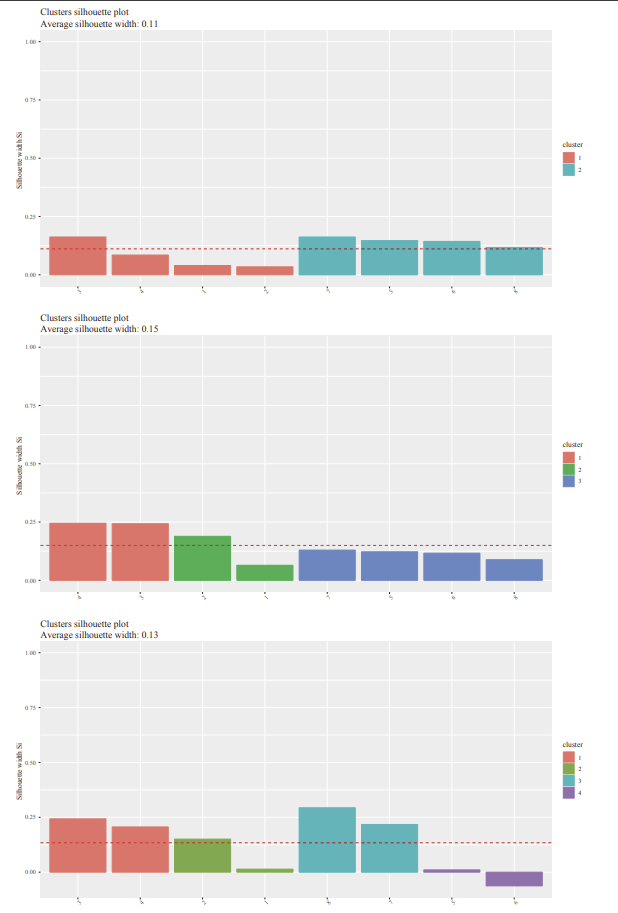
\includegraphics[width=0.8\textwidth]{chapter/chapter12/figure12_9.png}
\captionsetup{labelformat=empty}
\caption{\textbf{Figure 12.9:} Visualized silhouette information for three different clusterings of the same data set.}
\label{fig12.9}
\end{center}
\end{figure}

The function creates a dendrogram using one of the seven options for calculating the similarity of merged clusters. The options include average (unweighted pair-group arithmetic average method, UPGMA), single (single linkage), complete (complete linkage), ward (Ward's method), weighted (weighted average linkage, WPGMA), its generalization flexible which uses the Lance-Williams formula, and gaverage (a generalized average, flexible UPGMA using the Lance-Williams formula) [\cite{ref20}]. The default is the average option.

When the data to be clustered is not in a dissimilarity matrix, the similarities are calculated according to the metric parameter. It can be one of the following two values - euclidean for the Euclidean distance and manhattan for the Manhattan distance.

The agnes() function returns an object of class agnes with the components holding the information about the clustering results, such as the order of objects in a graphical plot (so the branches of the dendrogram do not cross), information about merging the clusters, a vector with the distances between merging clusters at the successive stages, and others.

An agnes object can be converted to a dendrogram using the pltree() function. Its parameters include an object of class twins (typically returned by functions agnes() or diana() returning objects that inherit from the twins class) that contains information about clustering, a title, labels for the clustered objects, and graphical parameters. The mandatory parameter is the first one, default values are used for the others (e.g., the labels for the clustered objects are derived from the first parameter).

\begin{verbatim}
\# finding a hierarchical clustering solution
hc <- agnes(distances)
\# taking first 25 characters of a document as a label
texts.labels <- paste(substr(texts, 1, 25), "...", sep="")
\# visualization of the clustering solution in a dendrogram
pltree(hc,
    hang=-1,
    main="Hierarchical clustering of documents",
    labels=texts.labels[hc\$order])
\end{verbatim}

The hang parameter describe how much below the rest of the plot the labels of the plot should hang. A negative value means that the labels are hanging down from 0 . The labels parameter assigns labels to the clustered objects.

A dendrogram visualizing agglomerative clustering of the eight documents can be found in Figure 12.10.

\begin{figure}[H]
\begin{center}
\captionsetup{labelformat=empty}
\caption{Hierarchical clustering of documents}
  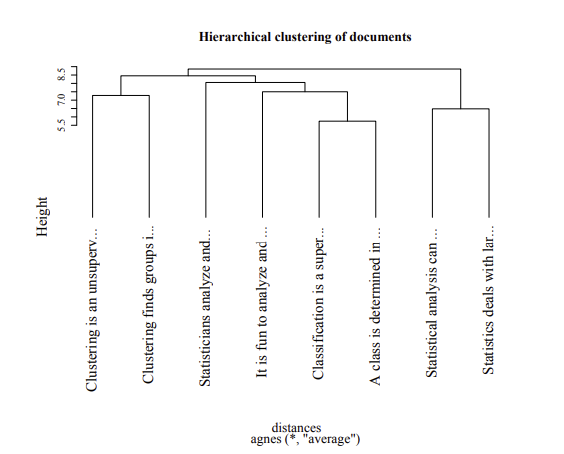
\includegraphics[width=0.7\textwidth]{chapter/chapter12/figure12_10.png}
\end{center}
\end{figure}

\textbf{Figure 12.10:} Visualized dendrogram for the agnes() method.

\begin{figure}[H]
\begin{center}
  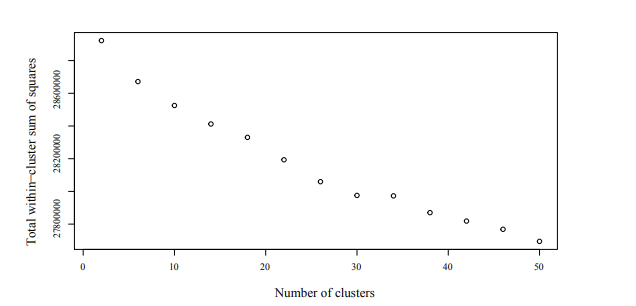
\includegraphics[width=0.7\textwidth]{chapter/chapter12/figure12_11.png}
\captionsetup{labelformat=empty}
\caption{\textbf{Figure 12.11:} The relationship between a number of clusters and the total within cluster sum of square errors when clustering 50,000 customer reviews from booking.com. An elbow is obvious for the number of clusters equal to 30 .}
\end{center}
\end{figure}

A divisive hierarchical algorithm is implemented by the diana() function (DIvisive ANAlysis). This algorithm starts with all items in one cluster. The clus-\\
ters are subsequently divided until each cluster contains only a single item. At each stage, the cluster with the largest diameter (the largest dissimilarity between any two of its observations) is selected.

The first parameter contains the data to be clustered. By default, it is again a dissimilarity matrix: a matrix, or data frame where each row represents one observation and each column a variable. The metric parameter, which can be one of the following two values - euclidean for the Euclidean distance and manhattan for the Manhattan distance is used to calculate dissimilarities.

The following example tries to find aspects of the hotel accommodation service, which is in fact an automatic detection of semantic content of groups of textual documents. The documents here are customer reviews written by people who really stayed in a hotel and have had real experience with it. The data comes from the famous server \href{http://booking.com}{booking.com} and a detailed description might be found in [\cite{ref295}]. In our experiment, 50,000 reviews written in Englsh were used in the analysis.

We can assume that similar documents share a common topic, in this case, an aspect of the service. To find groups of similar documents, clustering with the k -means algorithm was used. The elbow method analyzing the dependence between a number of clusters and the within cluster sum of square errors was used to find a right number of clusters needed by the k-means algorithm ( 30 clusters were chosen). Differential cluster labeling using the chi squared method (see Section 14.3.1 for details) was used to find representative words characterizing each cluster.

\begin{verbatim}
library(tm)
# reading the reviews and creating a document-term matrix
texts <- readLines("reviews-booking.txt")
documents <- data.frame(doc_id=1:length(texts),
            text=texts,
            stringsAsFactors=FALSE)
corpus <- Corpus(DataframeSource(documents))
corpus <- tm_map(corpus, removePunctuation)
corpus <- tm_map(corpus, content_transformer(tolower))
dtm <- DocumentTermMatrix(corpus,
    control=list(
        wordLengths=c(1, Inf),
        removeNumbers=TRUE,
        stopwords=TRUE,
        bounds=list(global=c(11, Inf)),
        weighting=function (x)
                weightSMART(x, spec="ntn")
\end{verbatim}

\begin{verbatim}
                )
)
mat <- as.matrix(dtm)
# calculating the within cluster sum of square errors for
# different numbers of clusters
withinss <- c()
for (k in seq(2, 50, 4)) {
        clustering <- kmeans(mat, k, iter.max=100)
        withinss[k] <- clustering$tot.withinss
}
# visualizing the relationship between a number of clusters
# and the within cluster sum of square errors to find an
# elbow denoting a suitable number of clusters
plot(withinss,
        xlab="Number of clusters",
        ylab="Total within-cluster sum of squares")
# 30 seems to be a good number of clusters
nclust <- 30
clustering <- kmeans(mat, nclust)
# calculating the values needed for Chi squared
# values estimation
D<-C<-B<-A<-matrix(nrow=nclust, ncol=dim(dtm) [2])
rownames(D)<-rownames(C)<-rownames(B)<-rownames(A)<-
                c(1:nclust)
colnames(D)<-colnames(C)<-colnames(B)<-colnames(A)<-
                colnames(dtm)
for (c in c(1:nclust)) {
    for (w in c(1:dim(dtm)[2])) {
        A[c,w] <- sum(dtm[clustering$cluster == c, w] != 0)
        B[c,w] <- sum(dtm[clustering$cluster != c, w] != 0)
        C[c,w] <- sum(dtm[clustering$cluster == c, w] == 0)
        D[c,w] <- sum(dtm[clustering$cluster != c, w] == 0)
    }
}
# calculating the values of the Chi square metric
# (not in one formula to prevent integer overflow due
# to very high numbers)
\end{verbatim}

\begin{verbatim}
chi <- dim(dtm)[1]*((A*D)-(C*B))^2
chi <- chi/(A+C)
chi <- chi/(B+D)
chi <- chi/(A+B)
chi <- chi/(C+D)
# calculating the average tf-idf of terms in the collection
avg_frequencies <- colMeans(mat)
# calculating the average tf-idf of terms in each class
tab <- rowsum(mat, clustering$cluster)
numbers_of_documents_in_clusters <- clustering$size
tab <- tab/numbers_of_documents_in_clusters
# printing 10 most important attributes for each class
# (only attributes with the average tf-idf value for a class
# higher than the average for all classes)
print("The values of Chi square for attributes and classes:")
for (c in c(1:nclust)) {
    print(paste("Class: ", c), sep="")
    print((sort((chi[c, tab[c, ] > avg_frequencies]),
        decreasing=TRUE)) [1:10])
}
# printing 5 documents closest to cluster centroids
for (c in c(1:nclust)) {
    print(paste("Cluster ", c, sep=""))
    distances <- apply(mat[c==clustering$cluster, ],
            1,
            function(x)
                sum((x - clustering$centers[c, ])^2)
            )
    print(texts[as.numeric(names(sort(distances)[1:5]))])
}
\end{verbatim}

The output of the statements above contains the list of the ten most discriminative words that are contained in documents from each cluster.

For some of the clusters, one can quite easily assign one clear label describing the main content well. For example, cluster 2 is about television, cluster 5 about indoor pool and gym, cluster 8 about airport shuttle. Other clearly identified aspects of the accommodation service include parking, credit cards, furniture,
expensive bar, beds, staff, etc. Examples of a few clusters with good labels follow (in fact, for most of the 30 clusters, a topic could be easily determined):
...\\[0pt]
[1] "Class: 2"


\begin{lstlisting}
[1] "Class: 2"
channels      tv           bbc          news         cnn
36592.5493    11672.0444   2430.7969    2413.2943    1566.8983
english       channel      language     digital      television
1221.4890     890.0239     496.8955     402.3057     267.6288
...

[1] "Class: 5"
pool          swimming     indoor       swim         gym
39290.3494    13360.0888   1395.6040    693.1596     515.0593
outdoor       spa          sauna        swiming      jacuzzi
484.8979      413.5477     367.6770     348.9054     334.2497
...

[1] "Class: 8"
airport       shuttle      taxi         bus          transfer
40243.6288    5033.6403    1259.5266    960.2551     758.1955
flight        close        fromto       driver       gatwick
727.6716      543.1865     486.8610     377.9844     346.0994
...

[1D "Class: 9"
dirty         carpet       carpets      sheets       stains
41349.3561    1481.7790    585.0428     446.2469     361.6065
filthy        bathroom     blood        cobwebs      wallpaper
337.5244      277.6227     275.5182     271.5584     248.0691
...

[1] "Class: 25"
parking       car          park         free         garage
29786.0432    7737.2175    4017.3253    805.5700     762.7539
space         spaces       secure       cars         difficult
710.4421      710.2466     579.6436     569.6599     335.8032
...
\end{lstlisting}



Of course, the results are not perfect. Therefore, there were some clusters for which one clearly defined topic could not be easily determined as shown below. Cluster 11 in this example, was quite big compared to the others, so further analysis of it could bring additional insights to the data.

\begin{lstlisting}
[1] "Class: 3"
friendly      staff        helpful      good         location
7854.677      7240.694     4325.775     4049.060     3163.018
excellent     clean        value        nice         great
2919.974      2852.039     1783.016     1656.075     1529.375
...

[1] "Class: 11"
improved friendliness    cleaness     cleaniness
   18.152680    14.861314    12.864497    11.573488
updating     convenience  closeness    victorian
   11.235698    8.744312     7.423451     7.086854
makeover     exciting
   7.042680     6.839037
...

[1] "Class: 13"
one           asked        get          said         told
2316.2821     1819.5886    1637.1390    1294.0469    1276.1080
night         another      even         got          day
1253.5418     1252.8707    1100.1629    1045.5220    985.9492
...
\end{lstlisting}

To get examples of whole documents from the clusters, the most typical were studied (most typical documents look close to the cluster centroids). Examples of such documents for several clusters can be found below.\\
\begin{verbatim}
[1] "Cluster 2"
[1] "Could have more TV channels"
[2] "Very good location..Very clean..friendly staff..English 
channels on TV"
[3] "No English channels on the TV."
[4] "TV channels are a bit fuzzy"
[5] "Just only few TV channels"
...
[1] "Cluster 5"
[1] "There is no pool"
[2] "the pool"
[3] "a pool"
[4] "That there was no pool"
[5] "absense of pool"
...
[1] "Cluster 8"
[1] "distence from airport"
[2] "location to shannon airport."
[3] "It was close to the airport!"
[4] "Very close to airport"
[5] "Close to Weeze Airport"
...
[1] "Cluster 9"
[1] "Dirty"
[2] "Toilet/Bathroom very dirty."
[3] "Dirty hotel"
[4] "Room was too small and dirty."
[5] "The hotel was very dirty& Room was very small"
...
[1] "Cluster 25"
[1] "Convient location,easy parking."
[2] "No Parking!"
[3] "no parking in the hotel"
[4] "Very good postion.easy parking"
[5] "The parking and location."
...
\end{verbatim}

% \include{sublogo}